
\section{Pre-Trained Models}\label{sec:app-models}
In this section we provide additional details on the models leveraged as prior knowledge by agents. 
Tables \ref{tab:obj_keypoints_hyperparams}, \ref{tab:vid_seg_hp}, \ref{tab:state_hp} report the hyperparameters used to train all models, the architecture presented in the original works is kept as the backbone of the models. 
Next, we provide a brief description of each model and the shape of their latent representation.
For spatial representation, the first dimension denotes the number of feature maps while the second and third dimensions denote the width and the height of each one.

\begin{itemize}
    \item \texttt{Video Object Segmentation} \citep{goel2018unsupervised}. This model takes as input the last two frames of the game and computes $K$ feature maps that highlight the moving objects. \\
    \textit{Embedding shape}: $[ 20 \times 84 \times 84 ]$.
    \item \texttt{State Representation} \citep{anand2019unsupervised}. Given the current state, it computes a linear representation exploiting the spatial-temporal nature of visual observations.\\
    \textit{Embedding shape}: $[512]$.
    \item \texttt{Object Keypoints} \citep{kulkarni2019unsupervised}. The model is composed of two heads that are used during inference: a convolutional network to compute spatial feature maps and a KeyNet \citep{jakab2018keynet} to predict the keypoints co-ordinates.\\
    \textit{Embedding shape}: CNN $[ 128 \times 21 \times 21 ]$, KeyNet $[ 4 \times 21 \times 21 ]$.
    \item \texttt{Deep Autoencoder}. It is used to encode the current state. It represents the context in attention-based combination modules like WSA and DPA. Its architecture is inspired by NatureCNN \citep{mnih2015human}.\\
    \textit{Embedding shape}: $[ 64 \times 16 \times 16]$.
\end{itemize}

\begin{table}[htbp]
    \begin{minipage}{.48\linewidth}
    \centering
        \begin{tabular}{ll}
            \multicolumn{1}{l}{\bf Hyperparameters}  &\multicolumn{1}{l}{\bf Value}
            \\ \hline \\
            Num. Tr. Envs & 10 \\ 
            Episodes & 1000 \\
            MAX ITER & 1e6 \\
            Batch Size & 64 \\
            Image Channels & 1 \\
            K & 4 \\
            Learning Rate  & 1e-3 \\
            Learning Rate Decay & 0.95 \\
            Learning Rate Deacy Len & 1e5 \\
            
        \end{tabular}
        \caption{Object keypoints hyperparameters \citep{kulkarni2019unsupervised}.} \label{tab:obj_keypoints_hyperparams}
    \end{minipage}%
    \hfill
    \begin{minipage}{.48\linewidth}
        \centering
        \begin{tabular}{ll}
            \multicolumn{1}{l}{\bf Hyperparameters}  &\multicolumn{1}{l}{\bf Value}
            \\ \hline \\
            Num. Frames & 2 \\ 
            Steps & 500.000 \\
            Batch Size & 64 \\
            Learning Rate  & 1e-4 \\
            Max Grad. Norm & 5.0 \\
            Learning Rate Deacy Len & 1e5 \\
            Optimizer & Adam \\
            K & 20 \\
        \end{tabular}
        \caption{Video object segmentation hyperparameters \citep{goel2018unsupervised}.} \label{tab:vid_seg_hp}
    \end{minipage}
\end{table}

\begin{table}[htbp]
    \centering
        \begin{tabular}{ll}
            \multicolumn{1}{l}{\bf Hyperparameters}  &\multicolumn{1}{l}{\bf Value}
            \\ \hline \\
            Image Width  & 160 \\
            Image Height & 210 \\
            Grayscaling & Yes \\
            Action Repetitions & 4 \\
            Max-pool over last N action repeat frames & 2 \\
            Frame Stacking & 4 \\
            % End of episode when life lost & Yes \\
            % No-Op action reset & Yes \\
            Batch size & 64 \\
            % Sequence Length (CPC) & 100 \\
            Learning Rate (Training) & 5e-4 \\
            Learning Rate (Probing) & 3e-4 \\
            Entropy Threshold & 0.6 \\
            Encoder training steps & 80000 \\
            Probe training steps & 30000  \\
            Probe test steps & 10000  \\
            Epochs & 100 \\
            Feature Size & 512 \\
            Pretraining-steps & 100000 \\
            Num Parallel Envs. & 8 \\
            
        \end{tabular}
        \caption{State representation hyperparameters \citep{anand2019unsupervised}.} \label{tab:state_hp}
\end{table}

\pagebreak


\section{Combination Modules Analysis} \label{sec:app-com-mod}
In this section, we provide additional insights about the results of the initial analysis. 
The experimental setup, outlined in Sections \ref{sec:exp_setup}-\ref{sec:init_exp}, structures a robust framework for evaluating the various combination modules.

As shown in Table \ref{tab:emb_siz_modules}, we explore a variety of configurations for each module, ensuring a comprehensive assessment of their performance. Figures \ref{fig:pong_concat_modules}, \ref{fig:mspacman_concat_modules}, and \ref{fig:breakout_concat_modules} illustrate the training performance of each agent, offering a visual representation of their learning trajectories. Early stopping was applied for agents who showed no improvement over multiple evaluations. 


% pong
\begin{figure}[ht]
    \centering
    \begin{subfigure}[b]{0.45\textwidth}
        \centering
        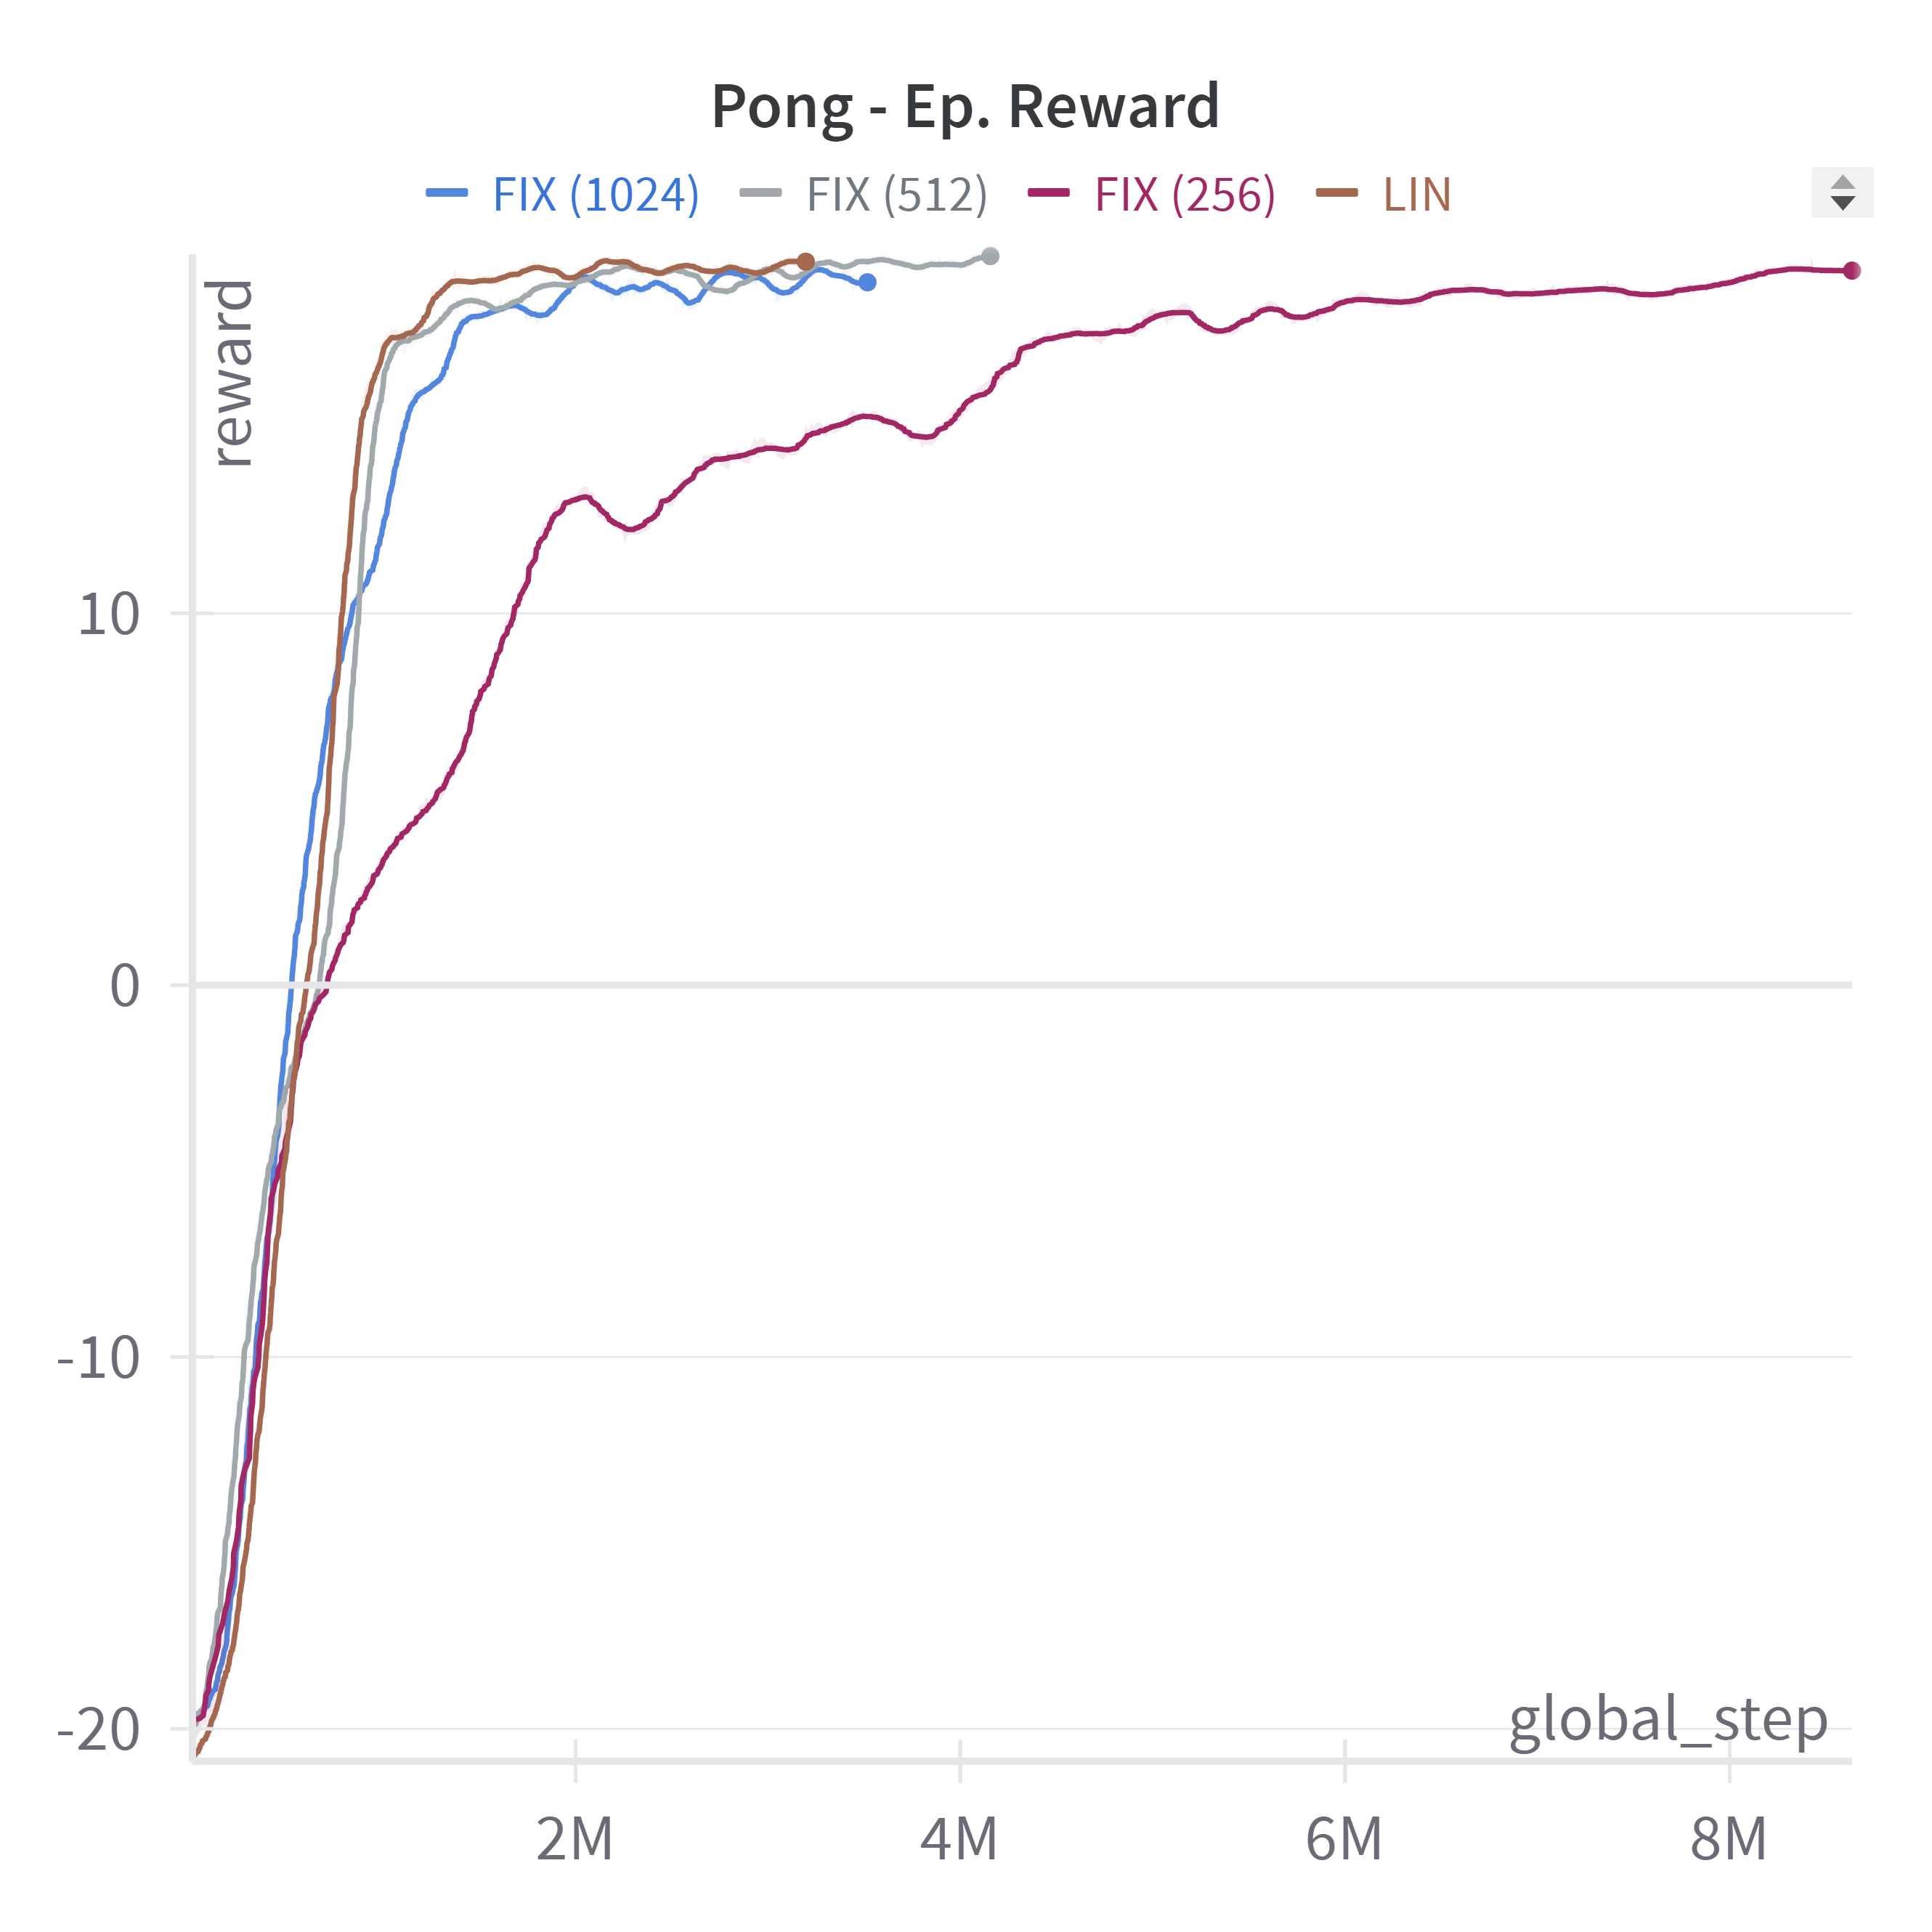
\includegraphics[width=\textwidth]{images/pong_lin_fix.png}
        \caption{\texttt{Linear} and \texttt{Fixed Linear}}
        \label{fig:pong_lin_fix}
    \end{subfigure}
    \hfill
    \begin{subfigure}[b]{0.45\textwidth}
        \centering
        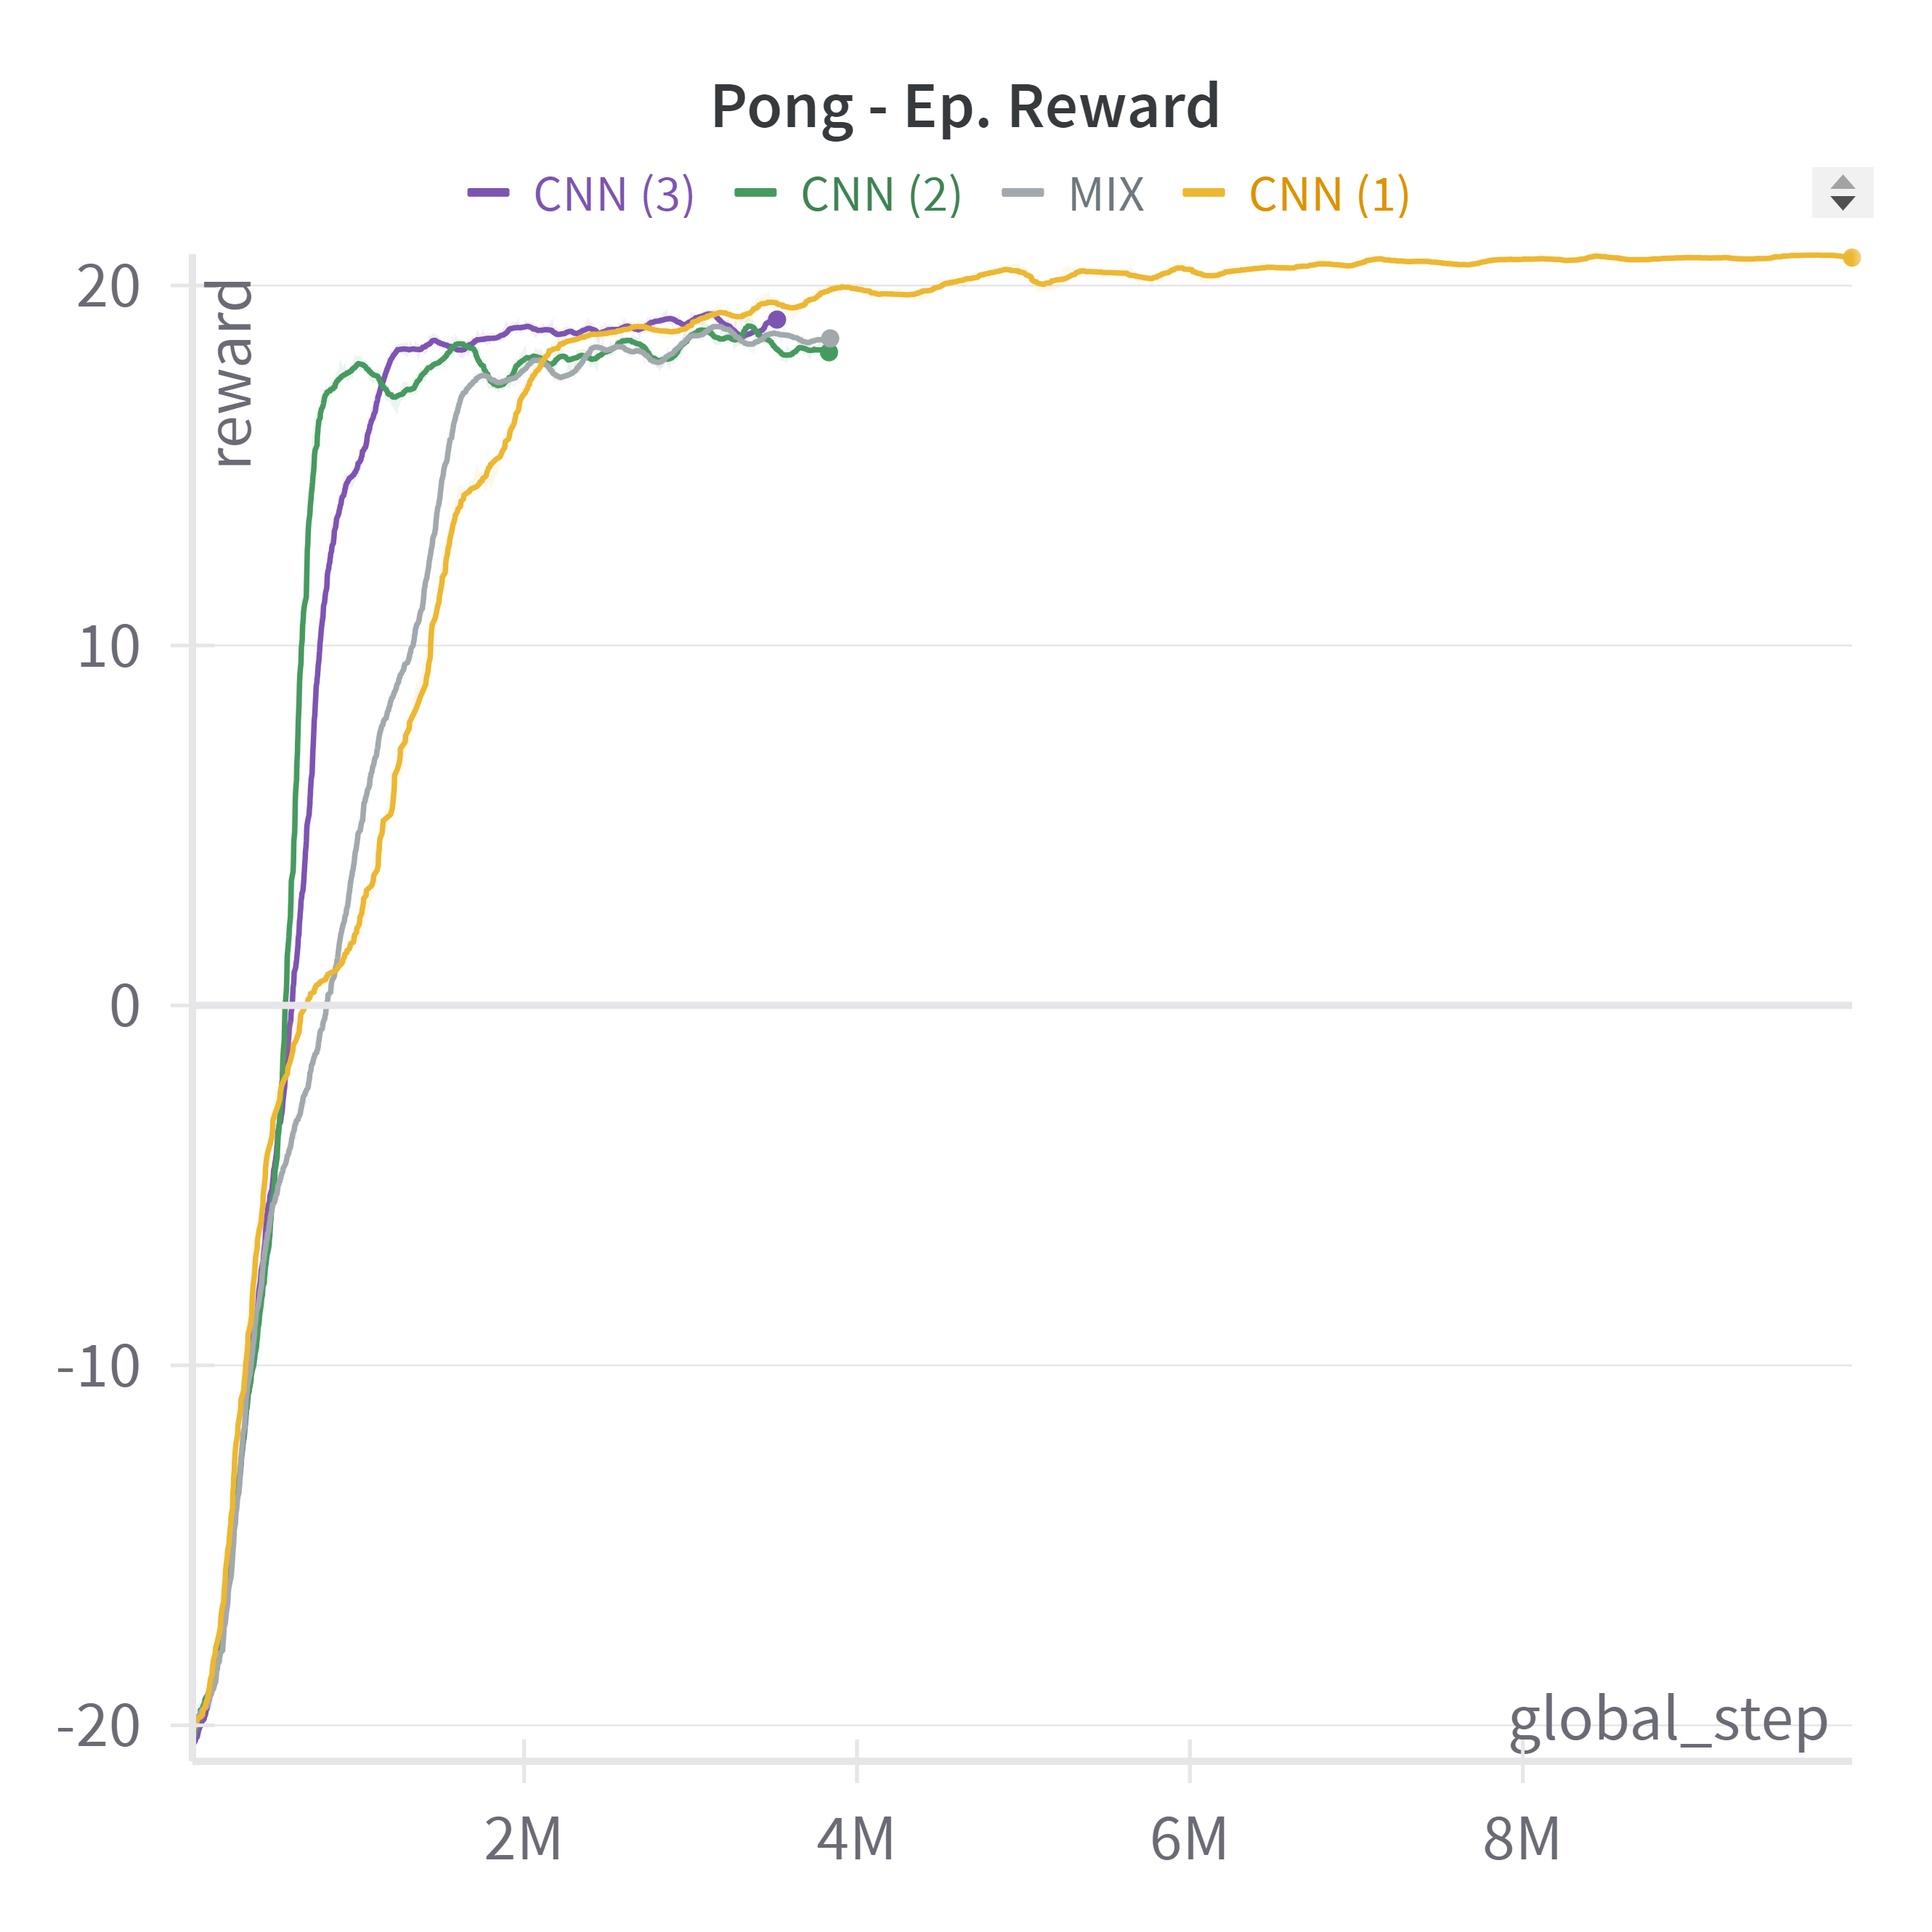
\includegraphics[width=\textwidth]{images/pong_cnn_mixed.png}
        \caption{\texttt{Convolutional} and \texttt{Mixed}}
        \label{fig:pong_cnn_mixed}
    \end{subfigure}
    \hfill
    \begin{subfigure}[b]{0.45\textwidth}
        \centering
        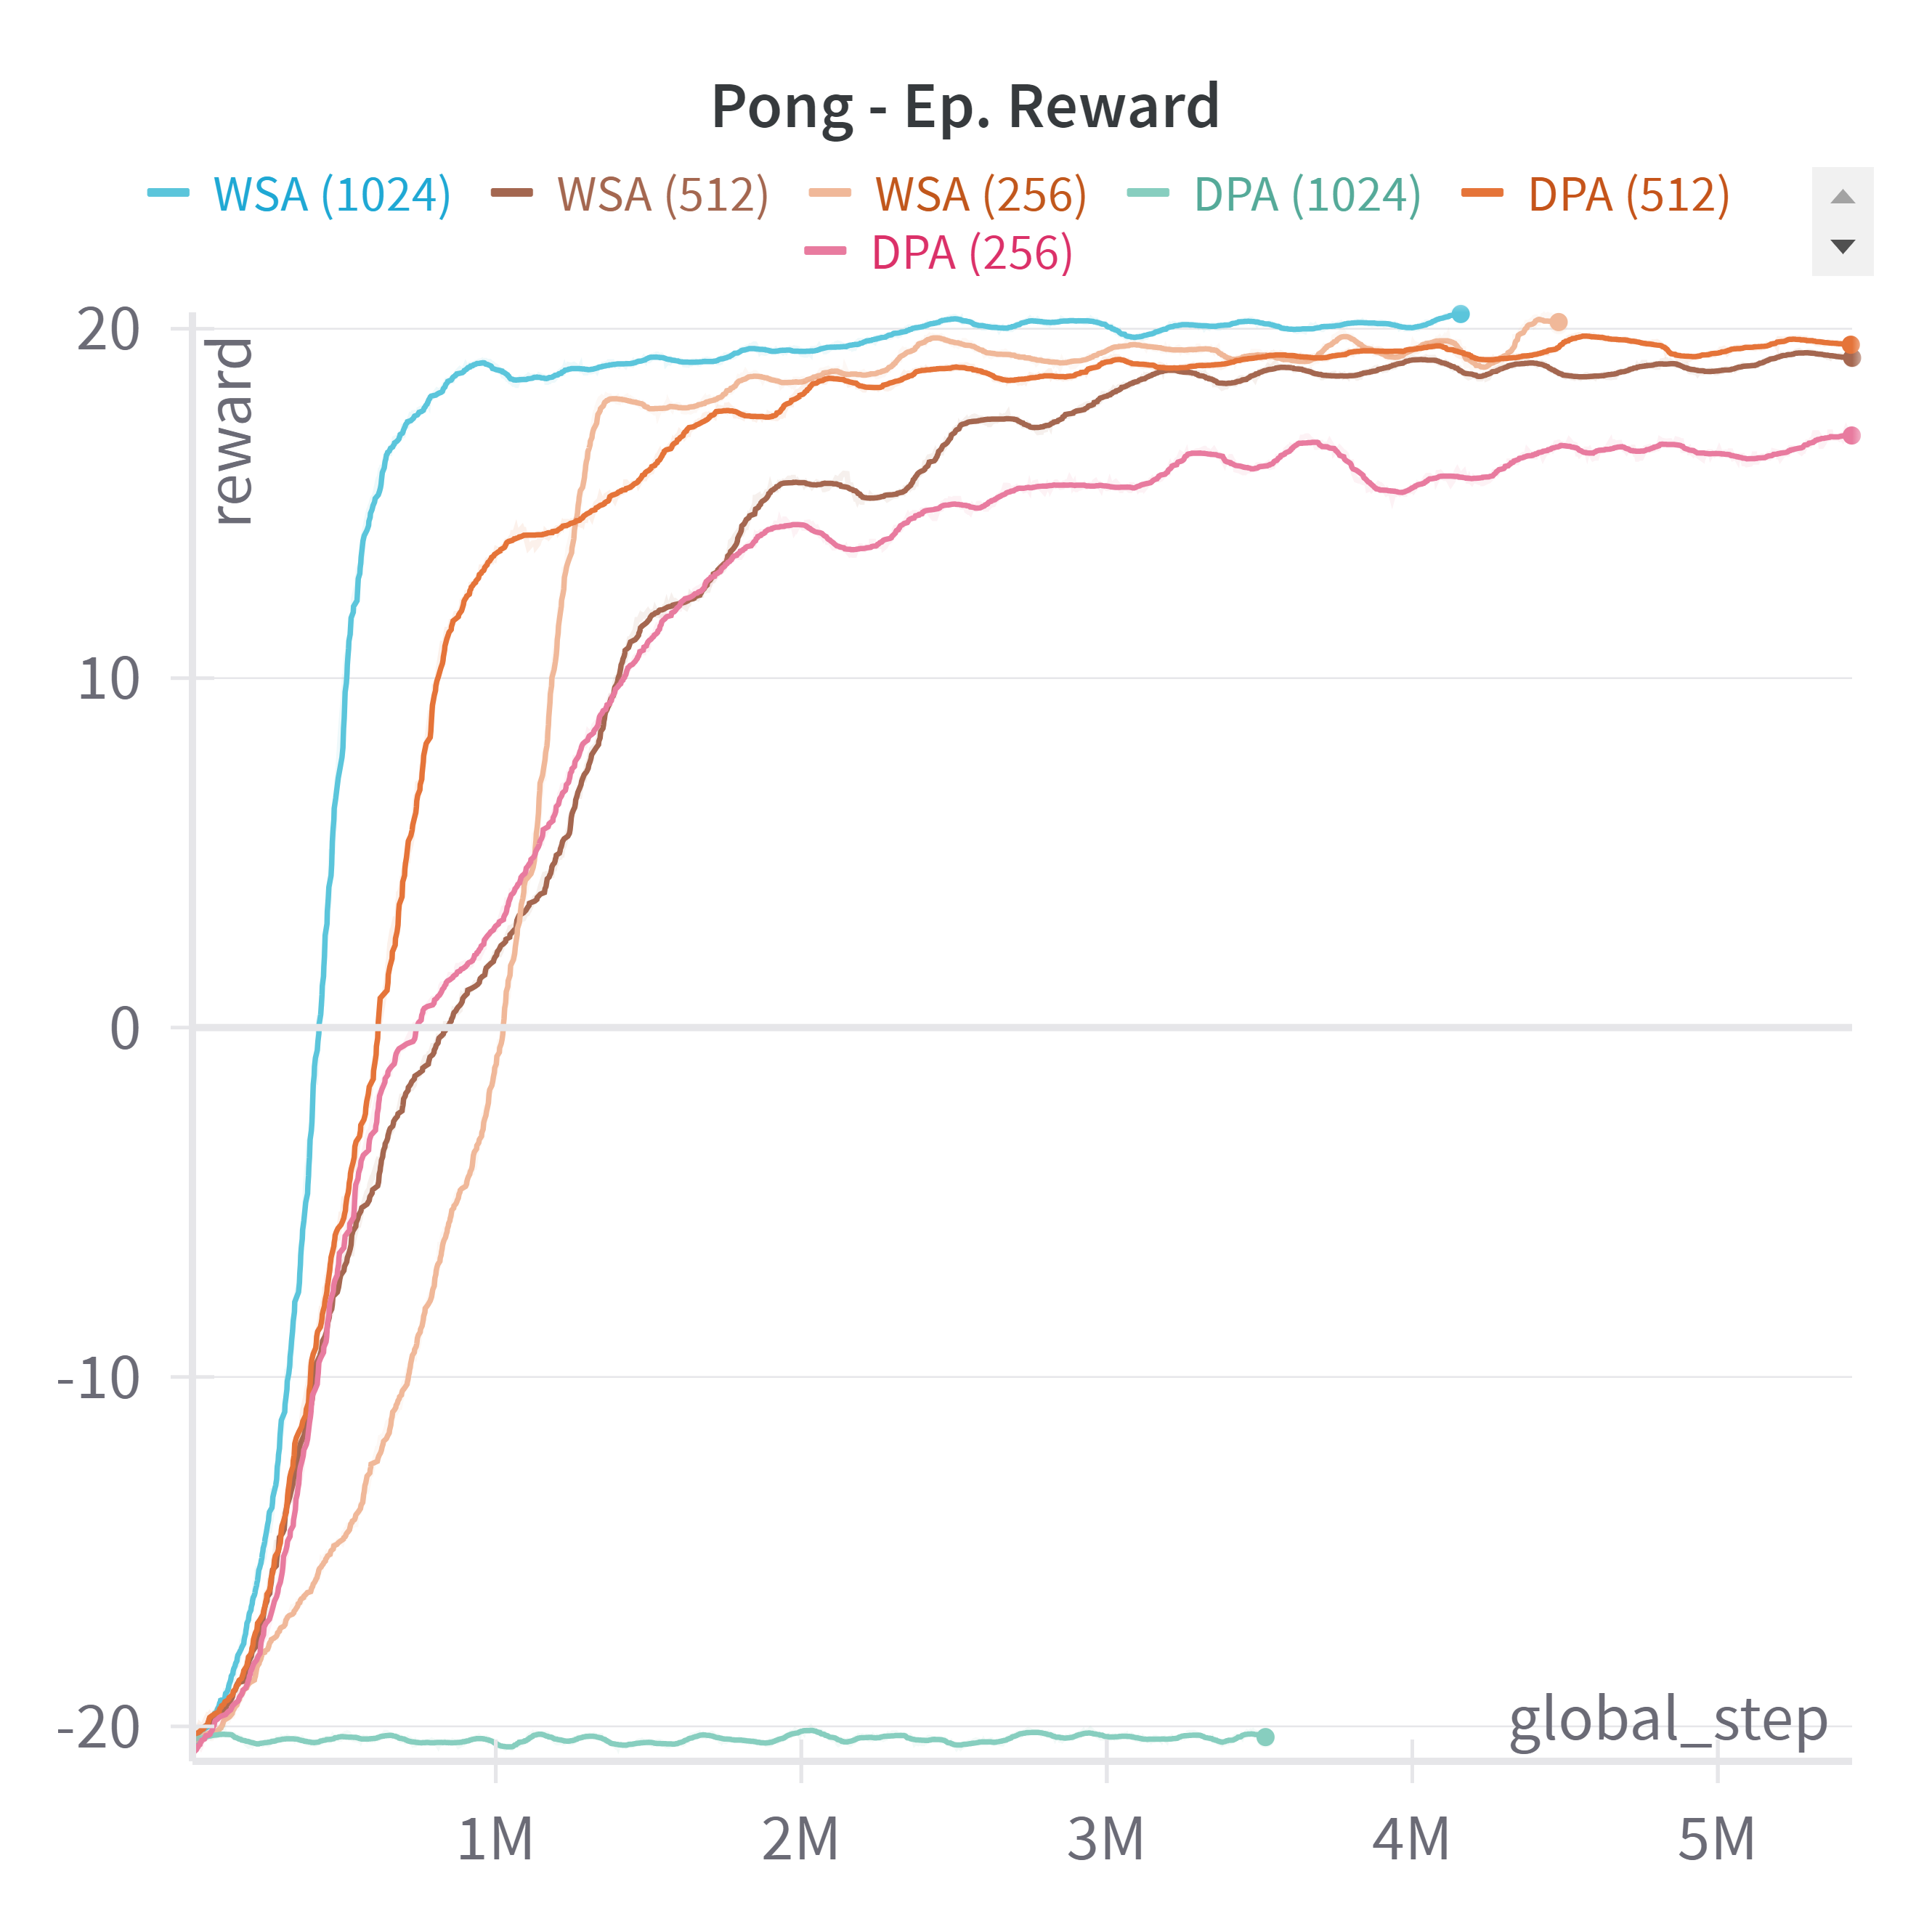
\includegraphics[width=\textwidth]{images/pong_wsa_dpa.png}
        \caption{\texttt{Weight Sharing Attention} and \texttt{Dot Product Attention}}
        \label{fig:pong_wsa_dpa}
    \end{subfigure}
    \hfill
    \begin{subfigure}[b]{0.45\textwidth}
        \centering
        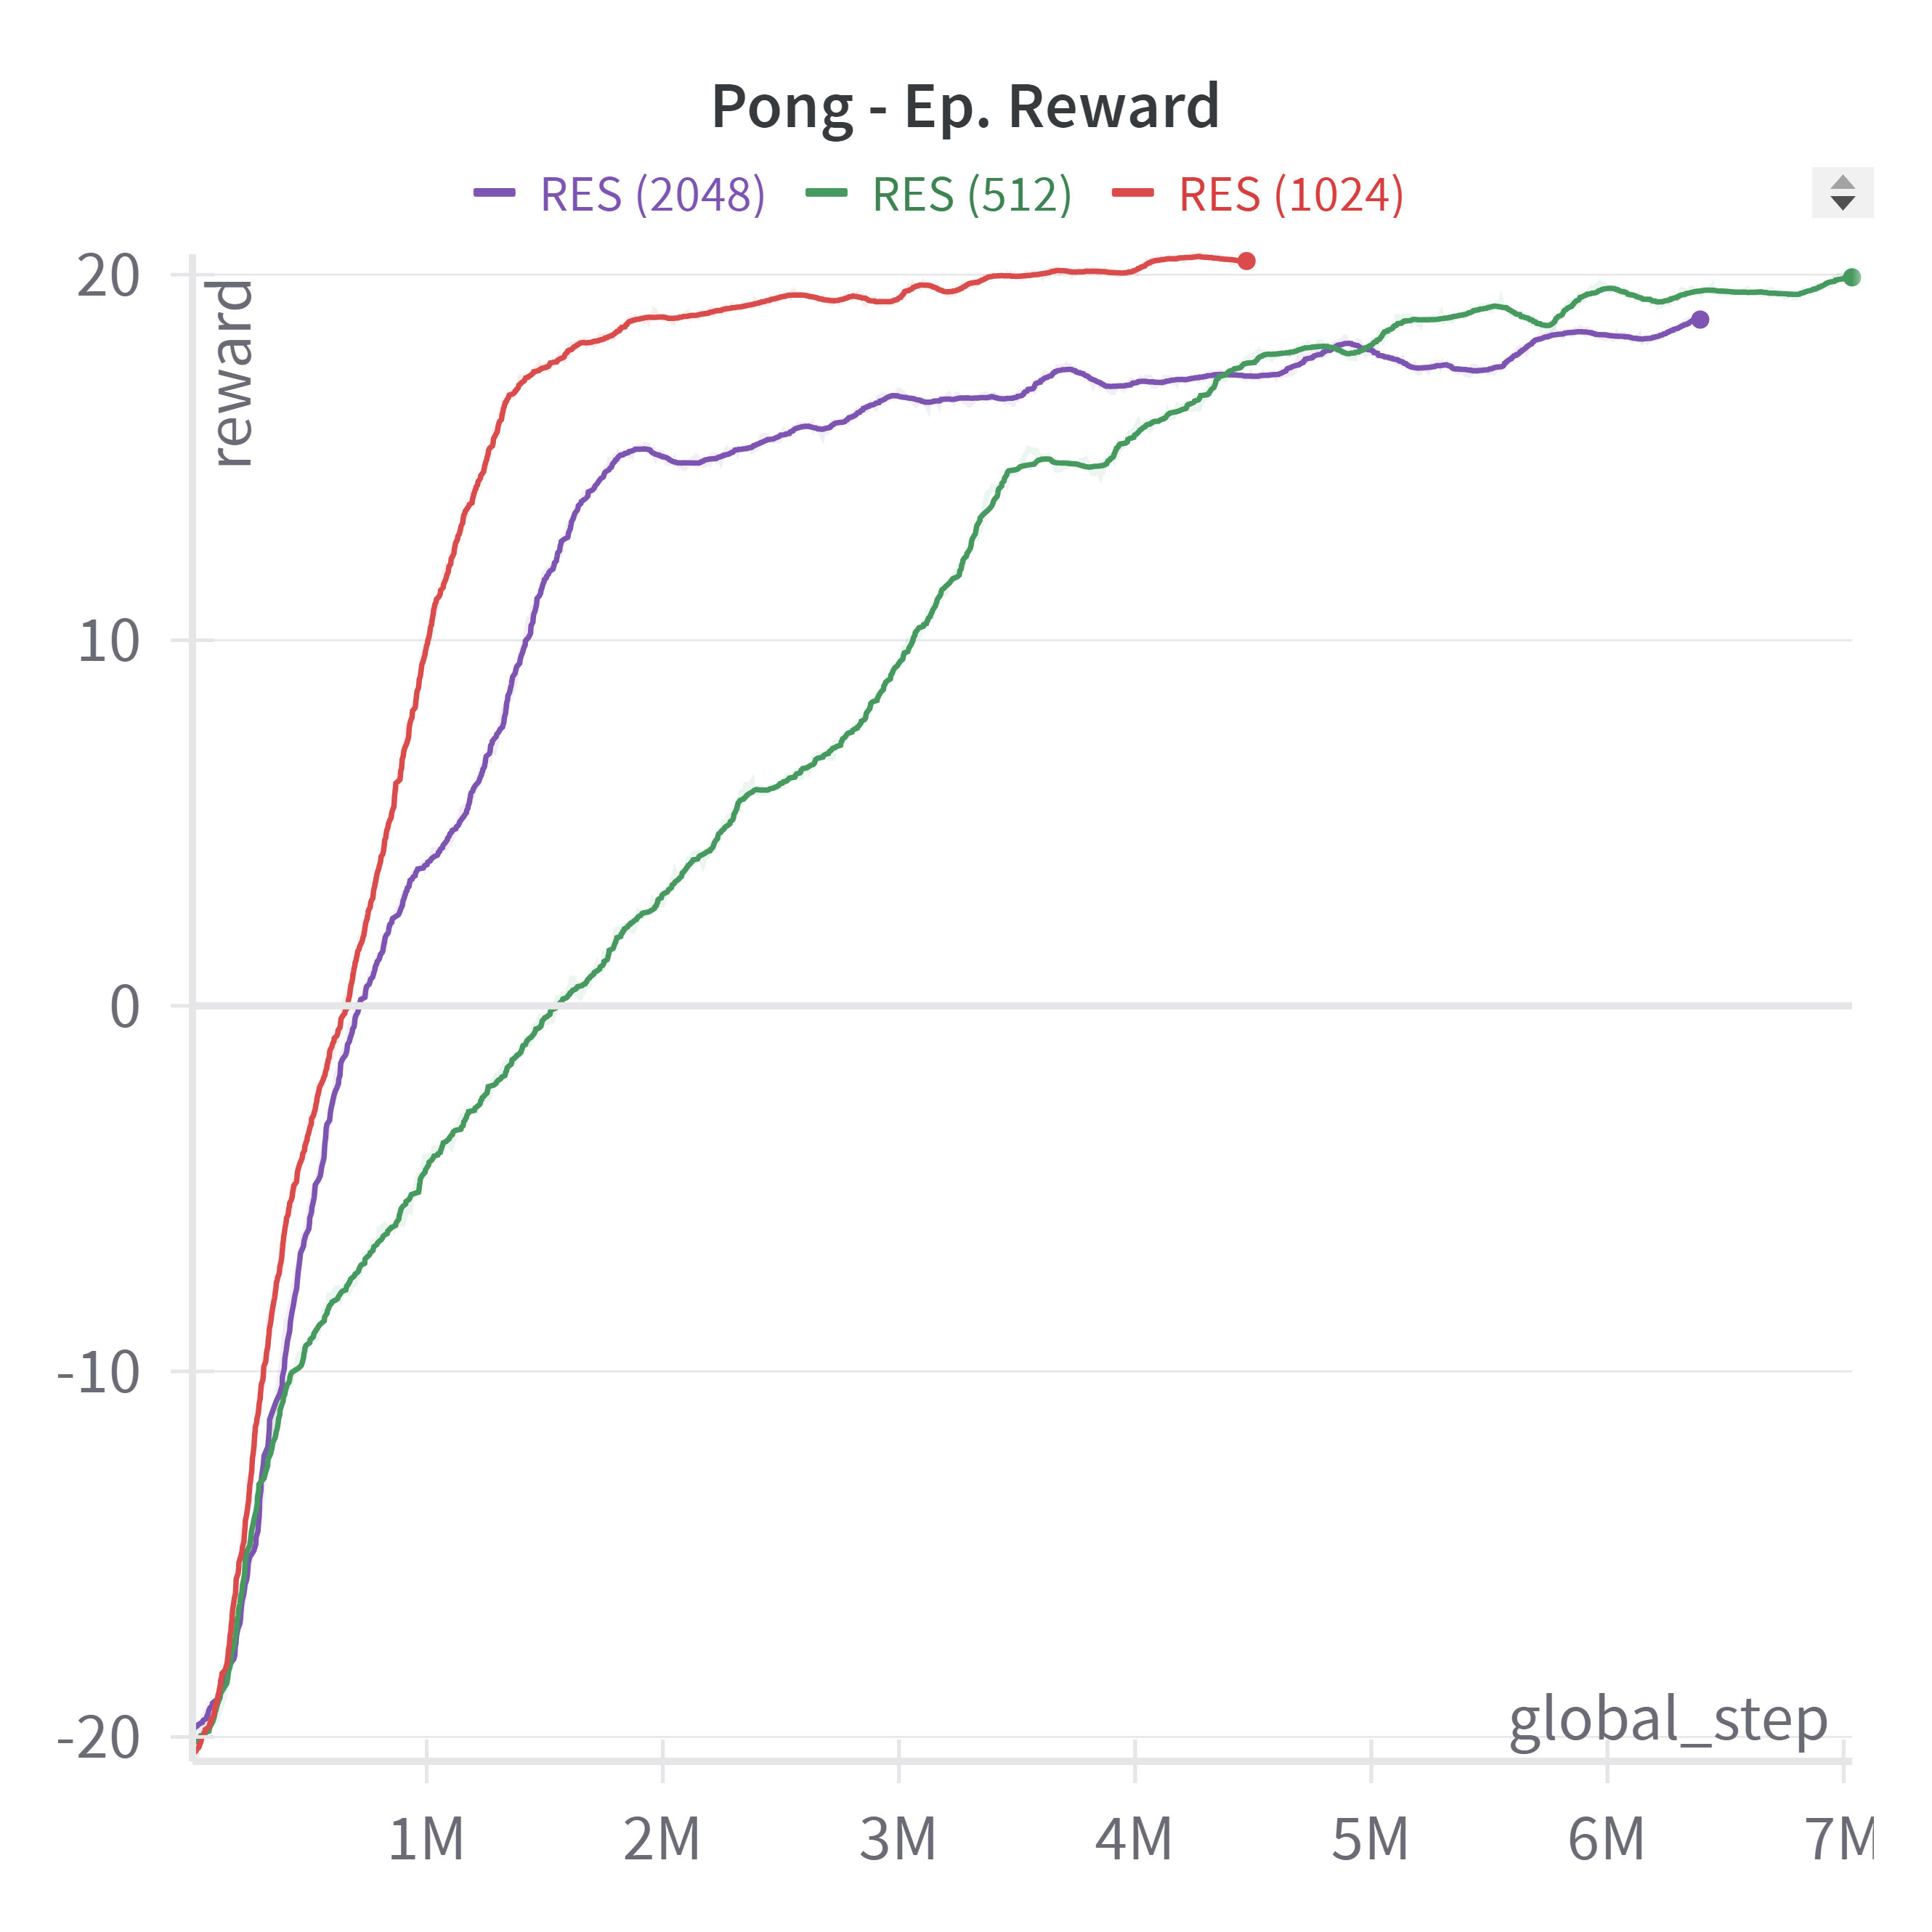
\includegraphics[width=\textwidth]{images/pong_res.png}
        \caption{\texttt{Reservoir}}
        \label{fig:pong_res}
    \end{subfigure}
    \caption{Initial analysis between different combination modules configurations on \texttt{Pong}.}
    \label{fig:pong_concat_modules}
\end{figure}

\begin{figure}[ht]
    \centering
    \begin{subfigure}[b]{0.45\textwidth}
        \centering
        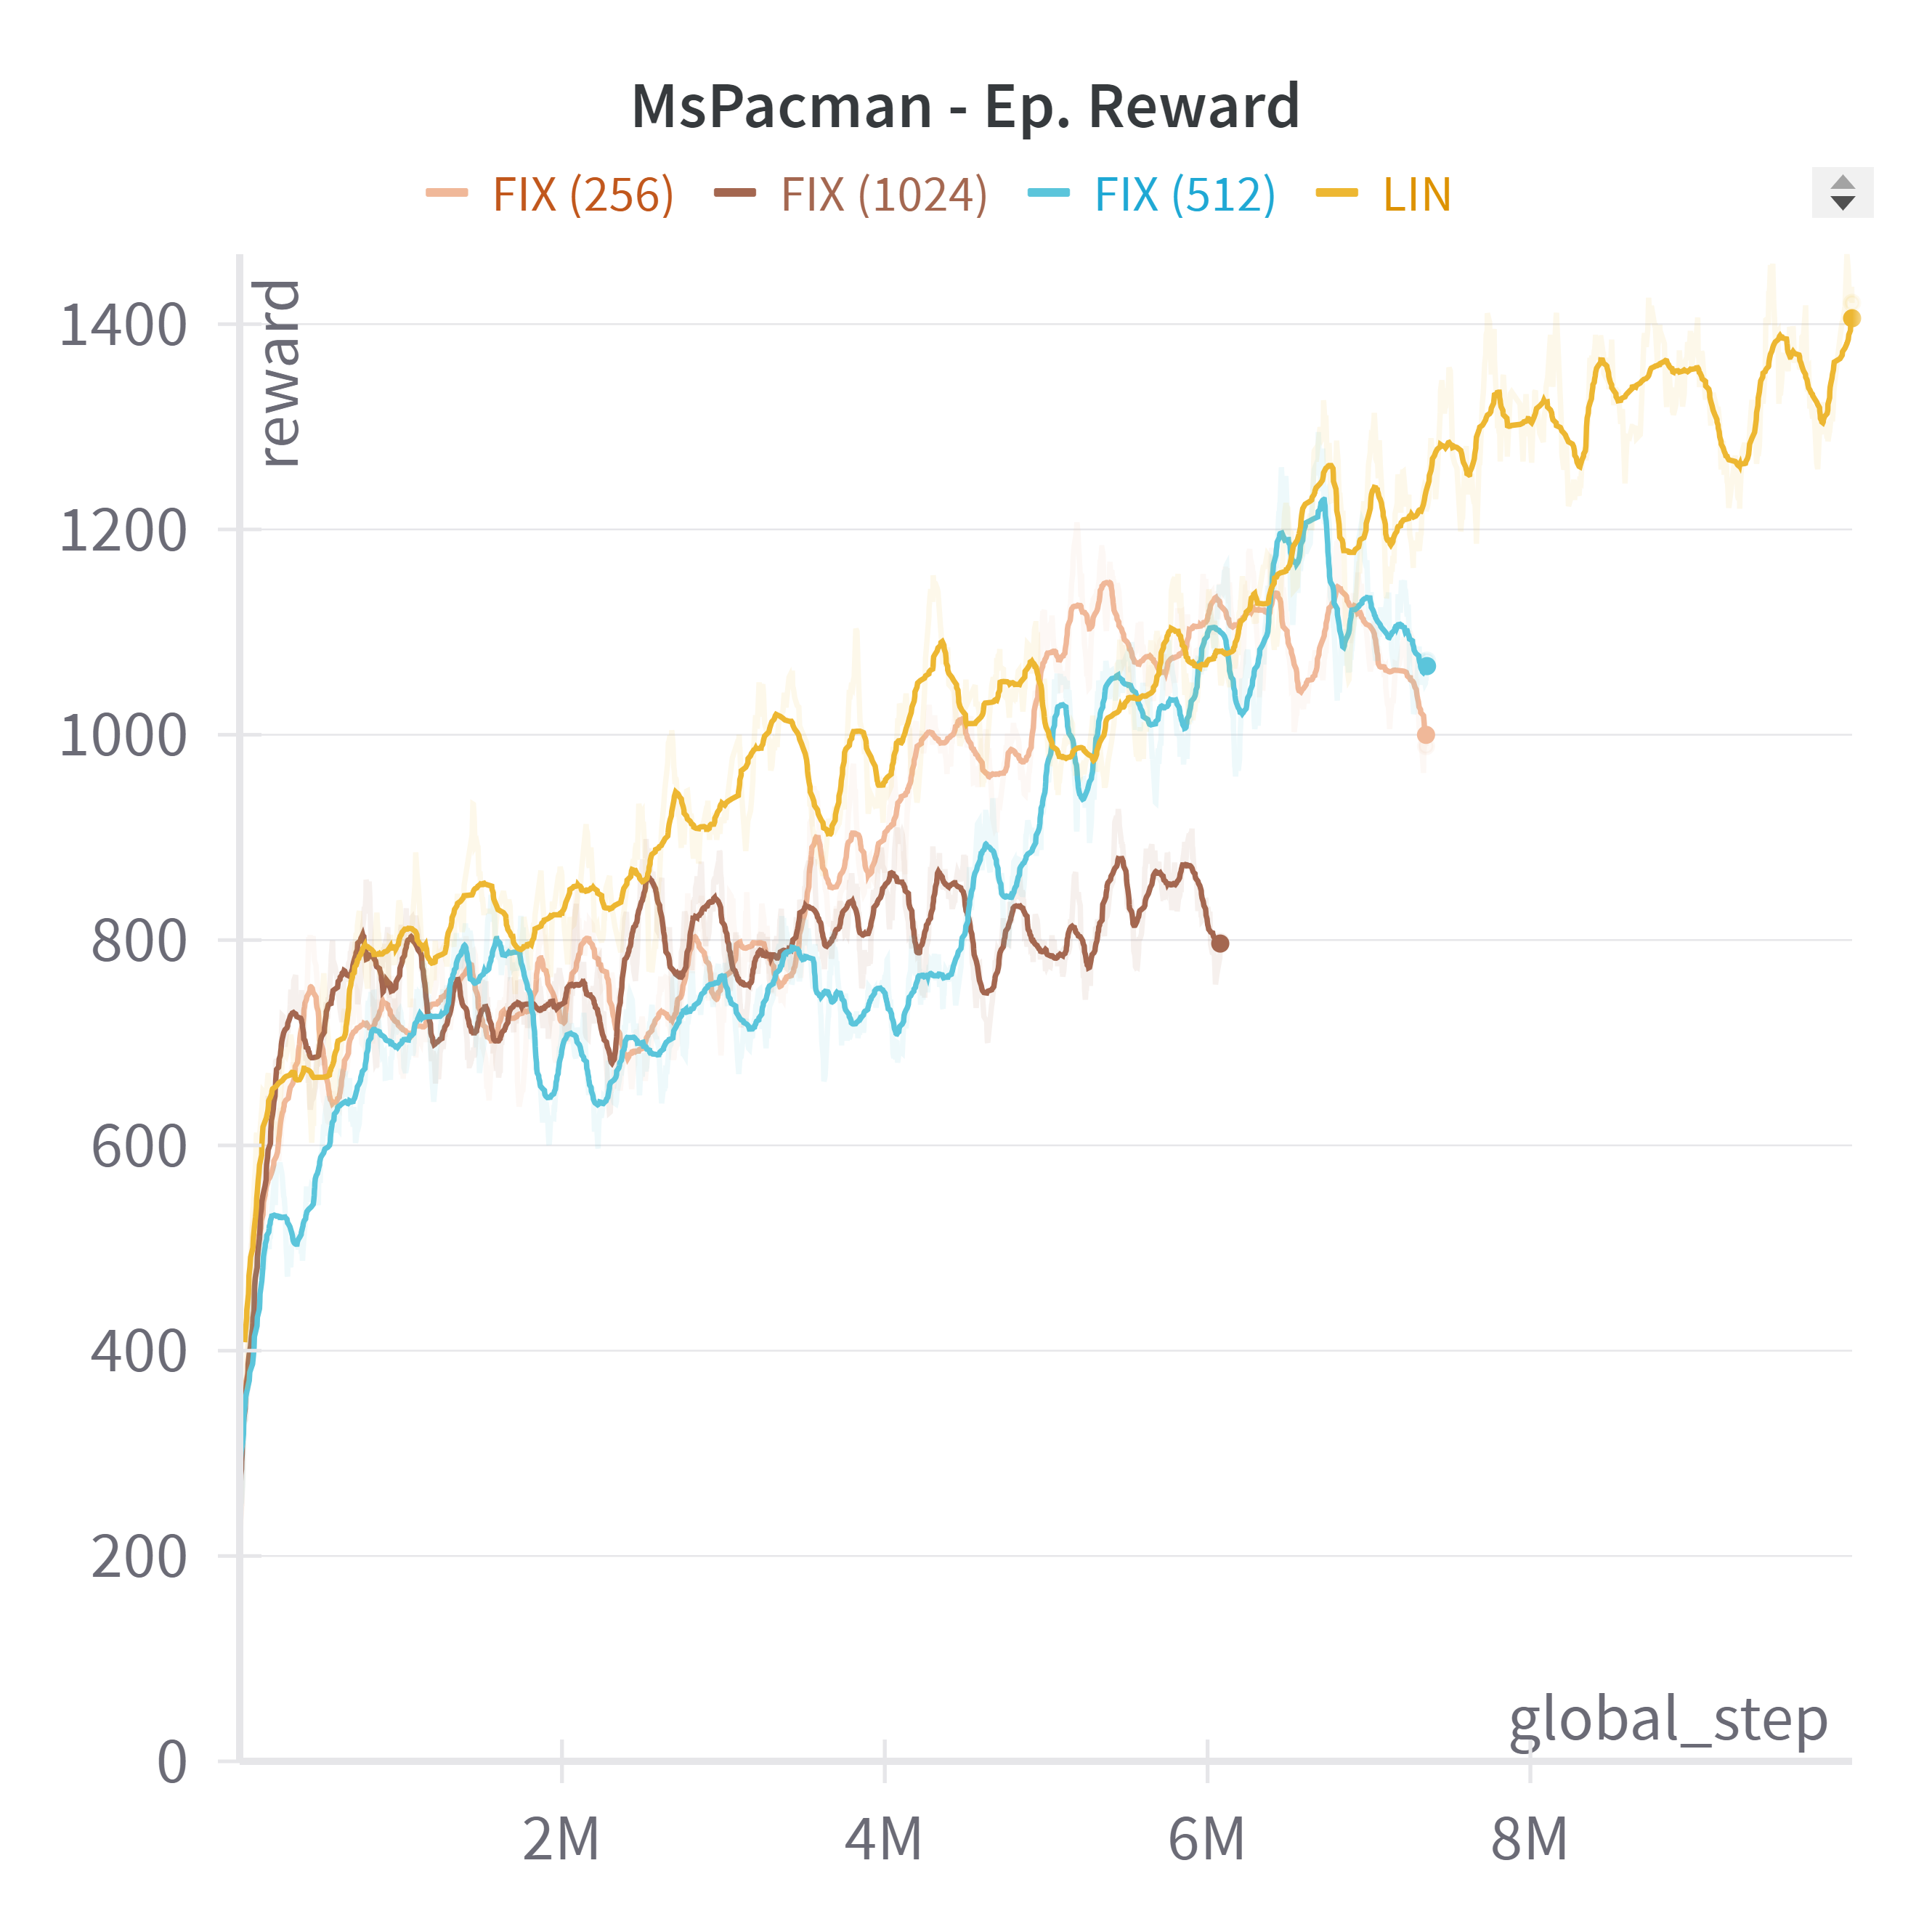
\includegraphics[width=\textwidth]{images/mspacman_lin_fix.png}
        \caption{\texttt{Linear} and \texttt{Fixed Linear}}
        \label{fig:mspacman_lin_fix}
    \end{subfigure}
    \hfill
    \begin{subfigure}[b]{0.45\textwidth}
        \centering
        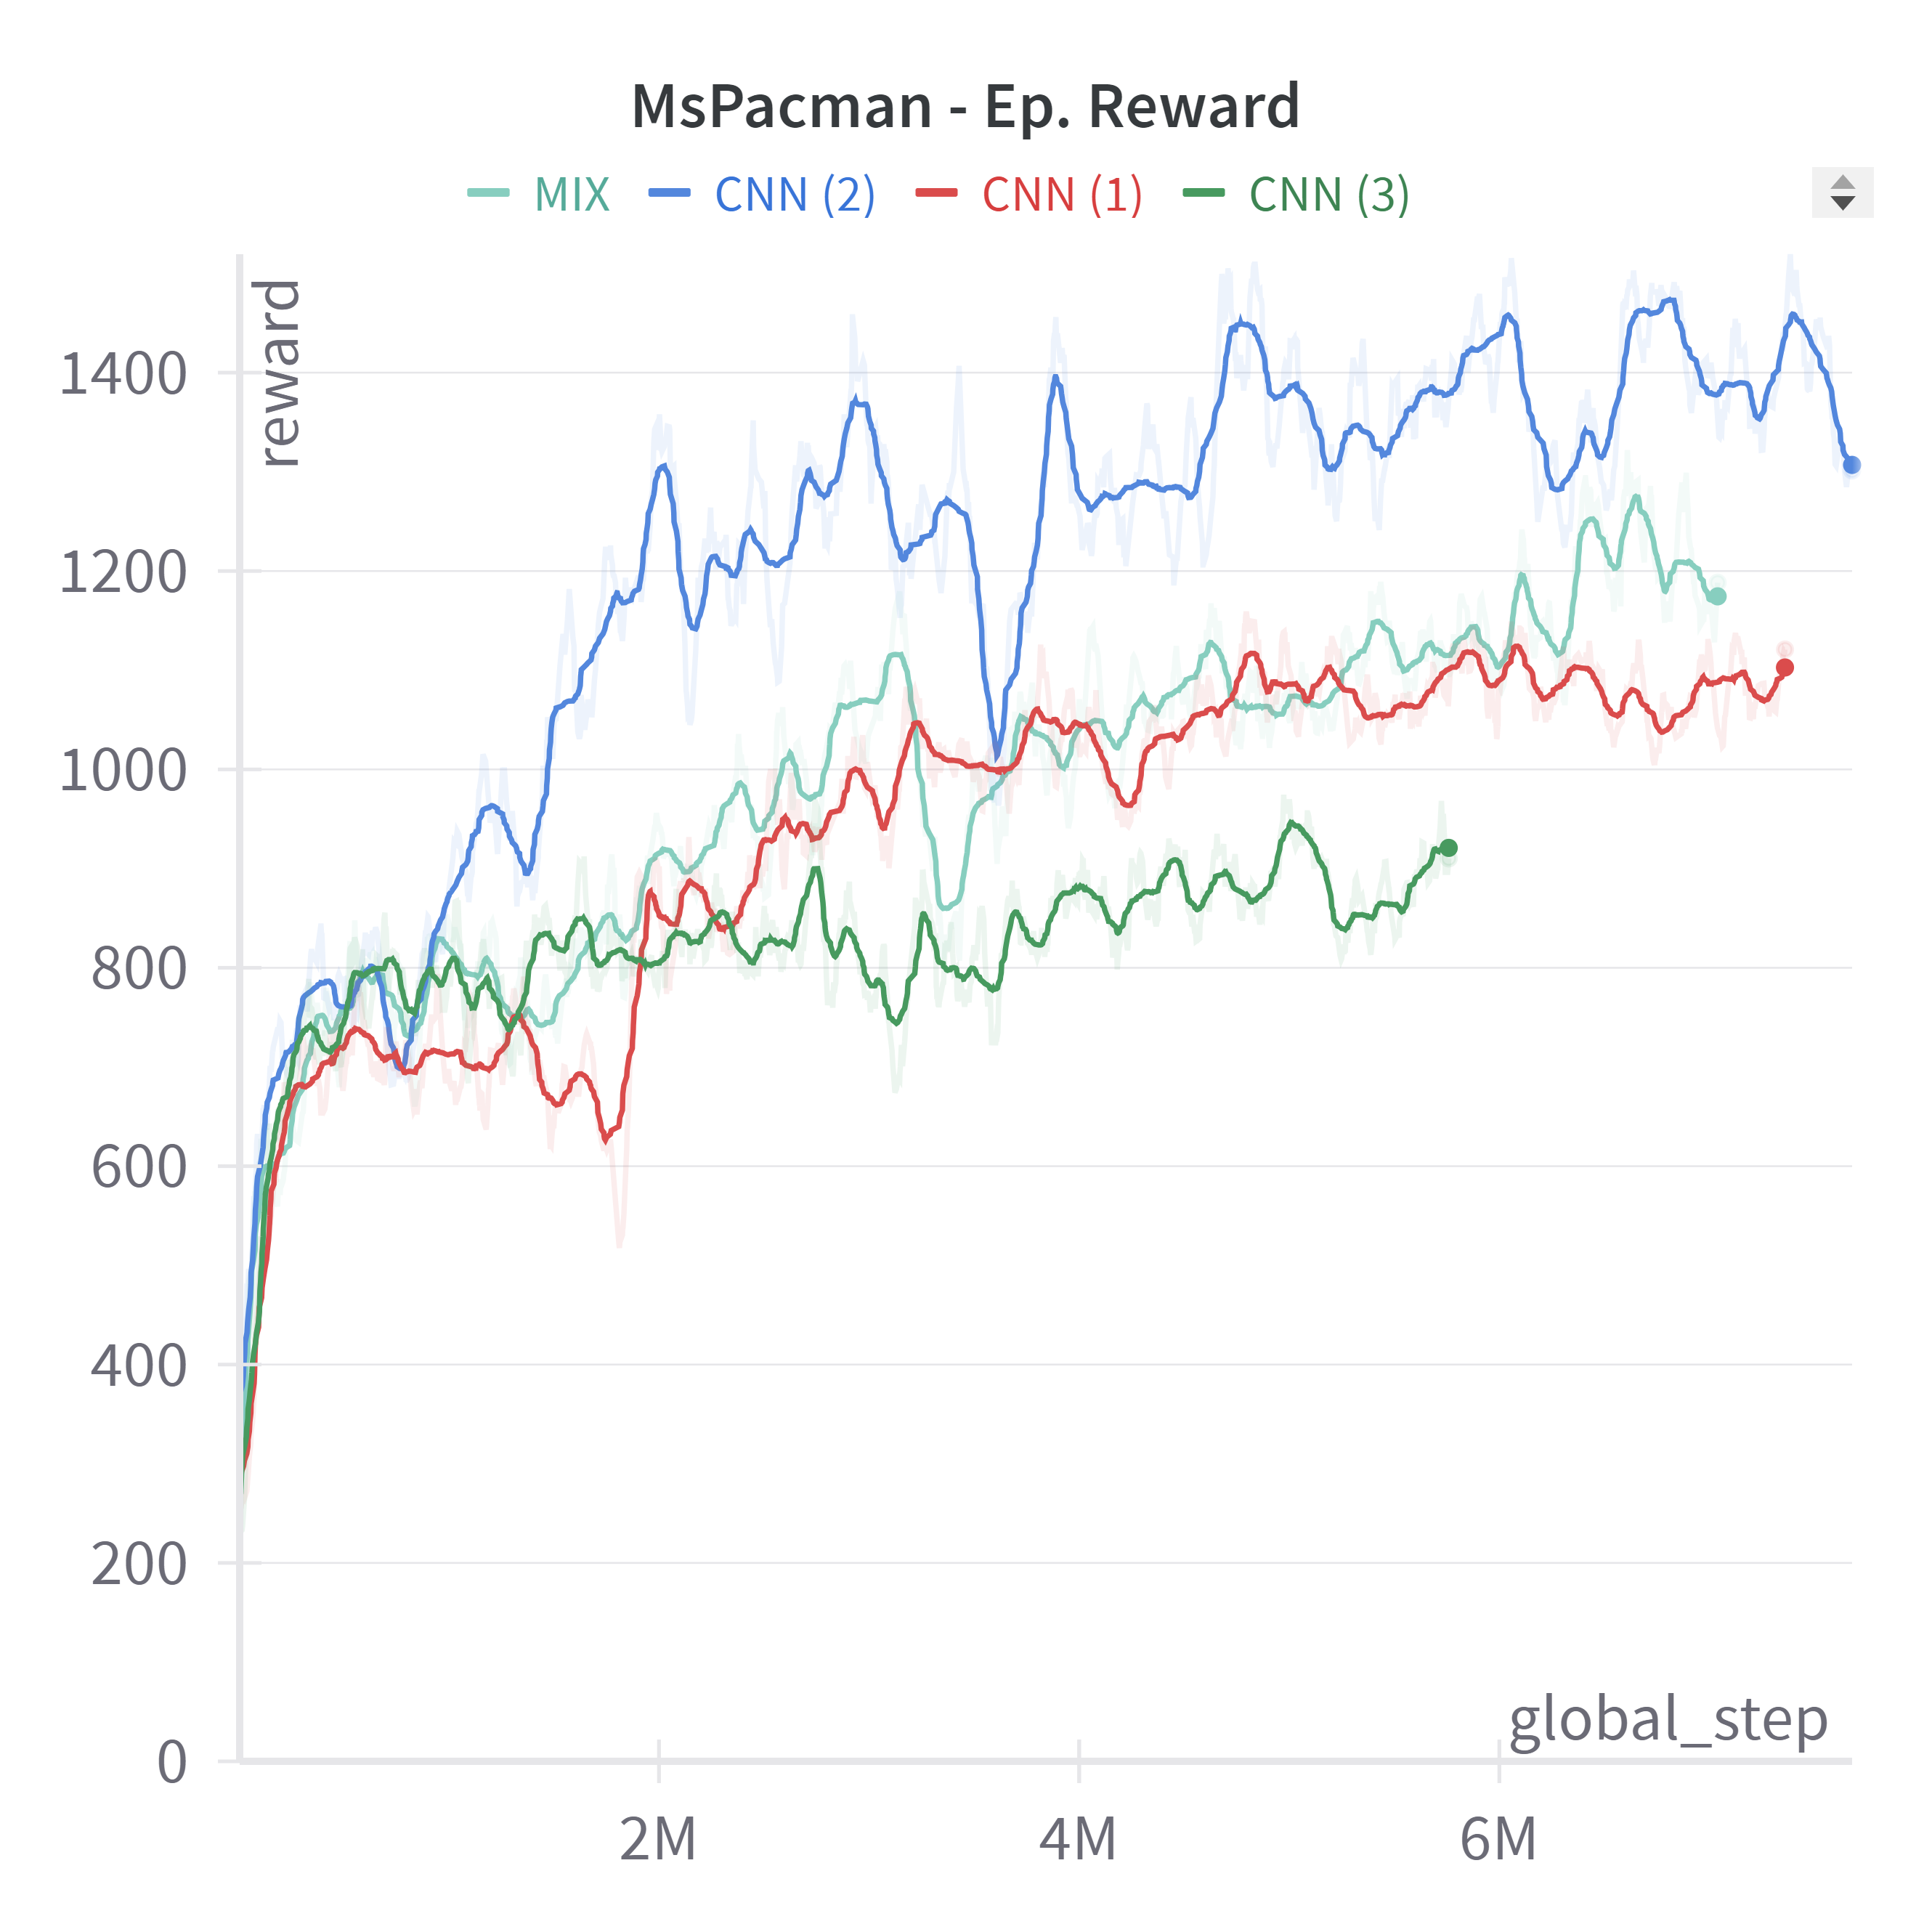
\includegraphics[width=\textwidth]{images/mspacman_cnn_mixed.png}
        \caption{\texttt{Convolutional} and \texttt{Mixed}}
        \label{fig:mspacman_cnn_mixed}
    \end{subfigure}
    \hfill
    \begin{subfigure}[b]{0.45\textwidth}
        \centering
        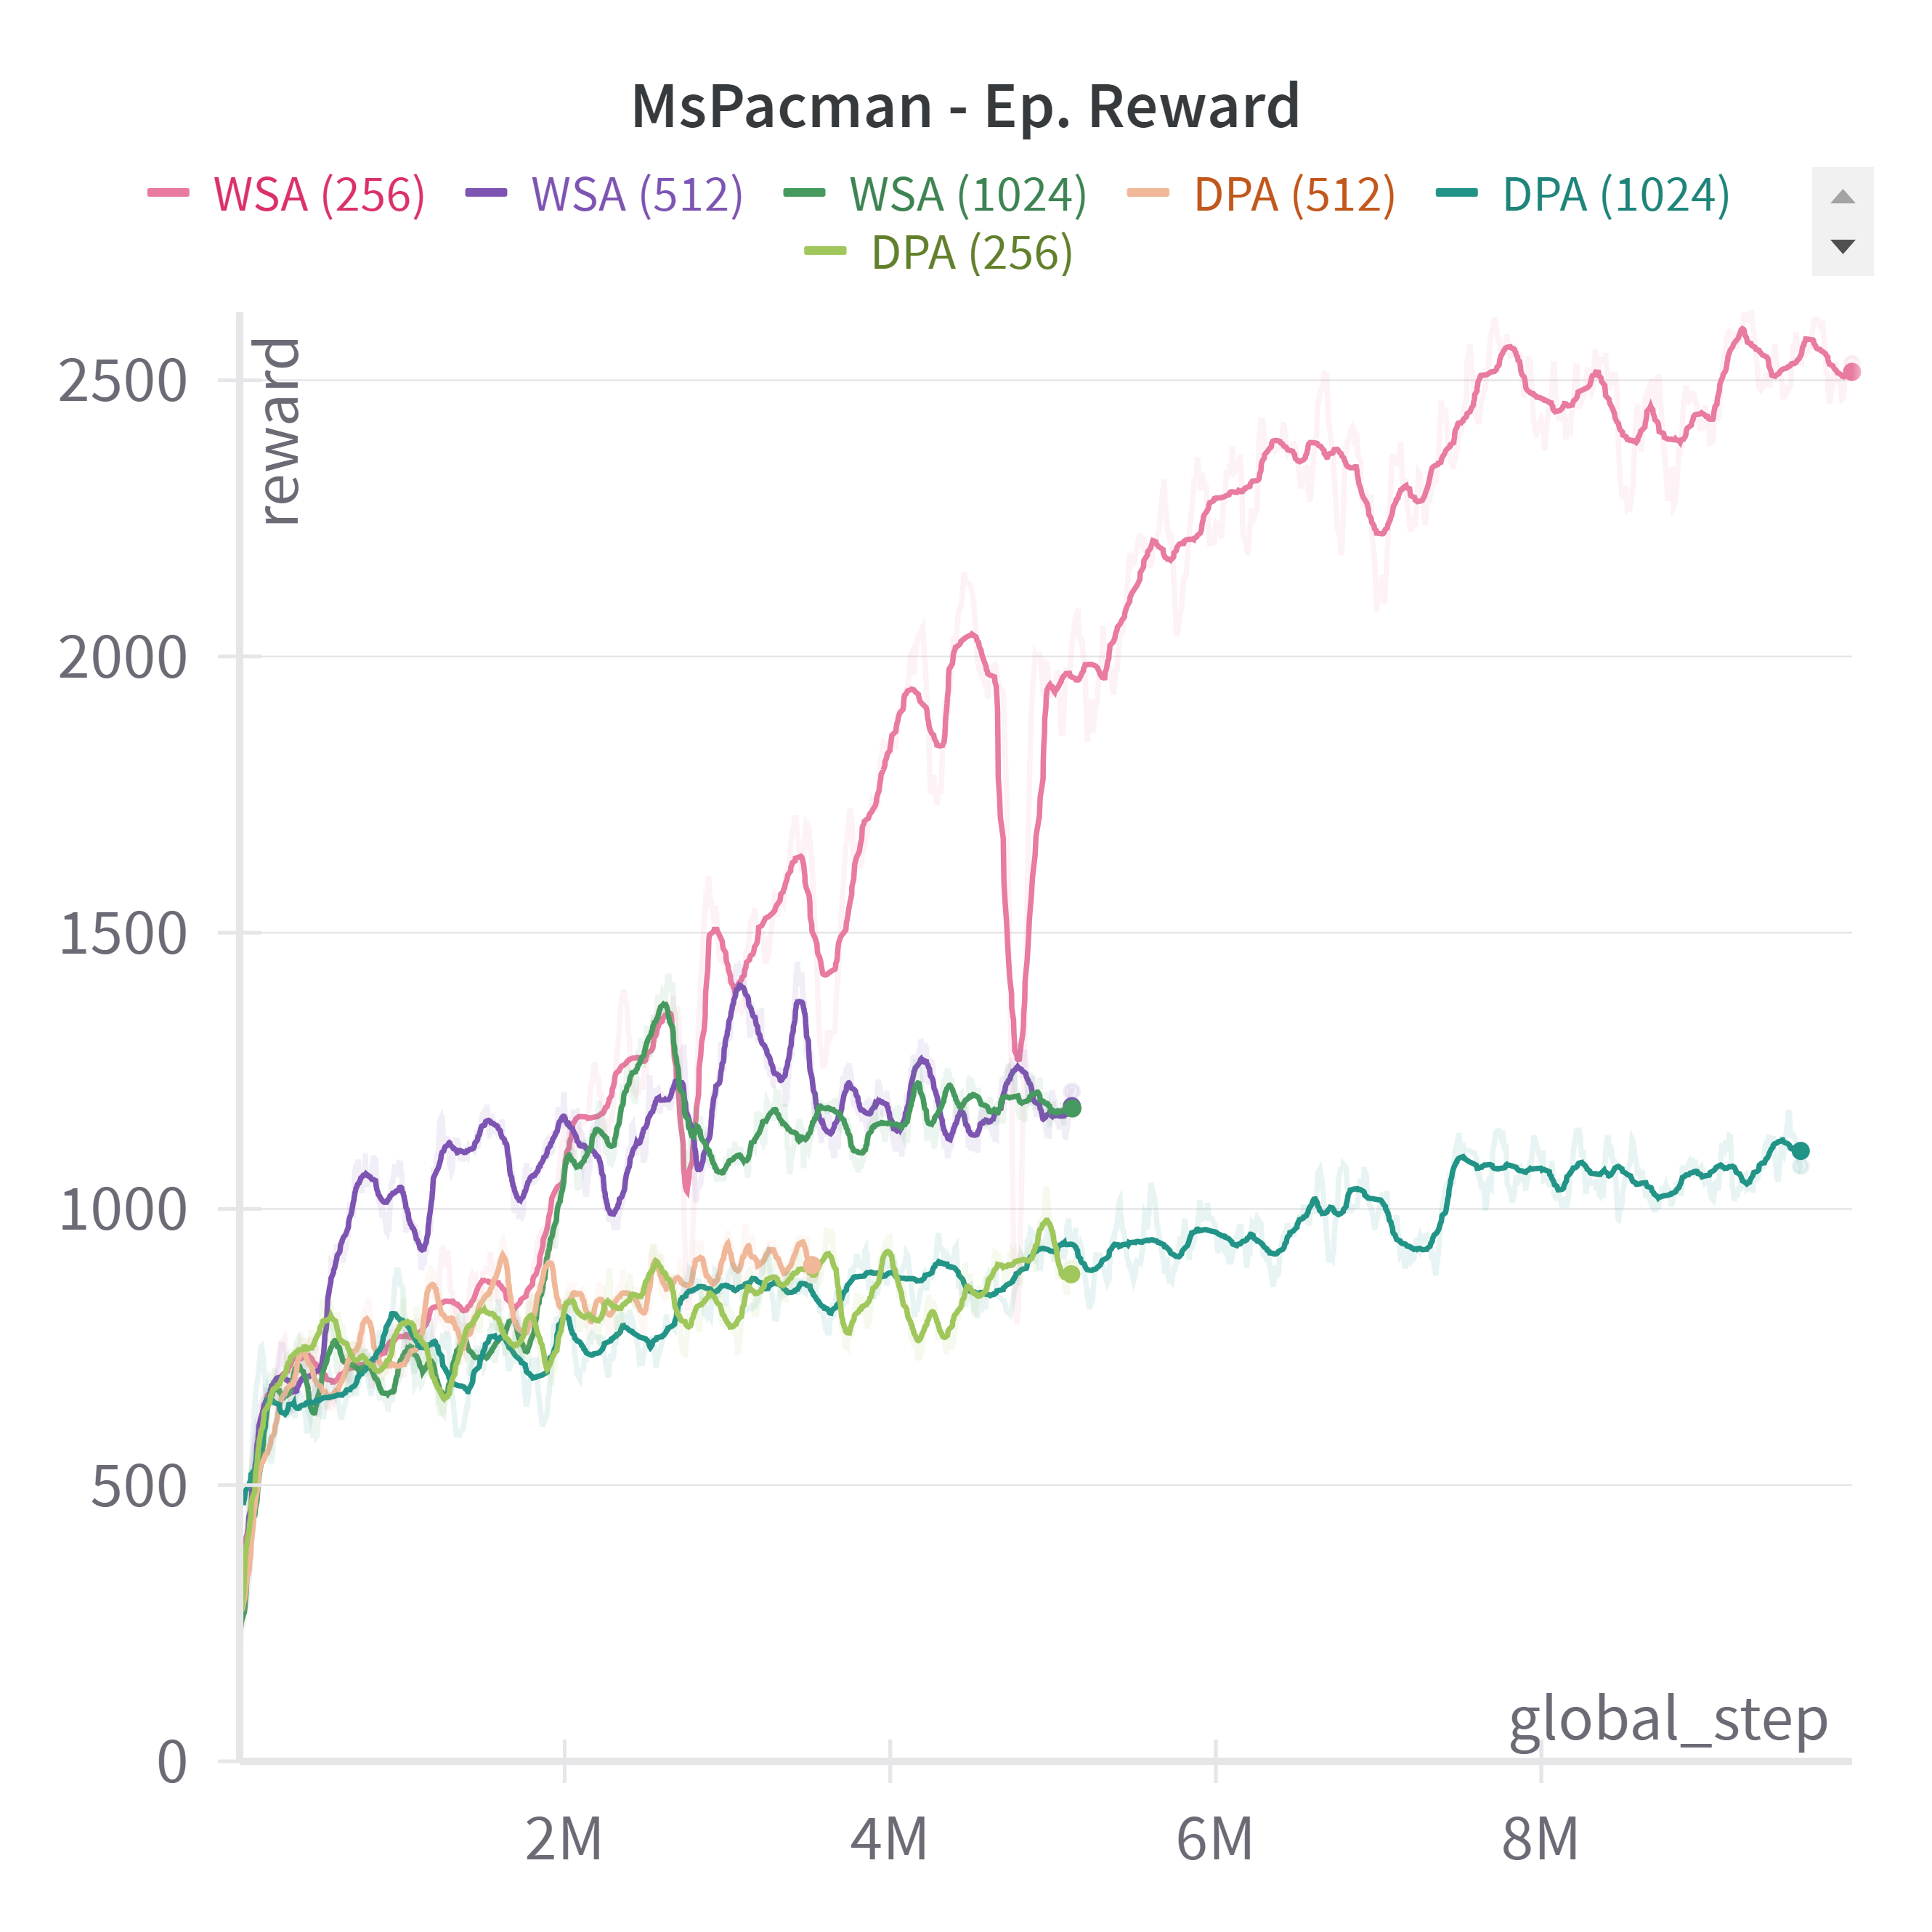
\includegraphics[width=\textwidth]{images/mspacman_wsa_dpa.png}
        \caption{\texttt{Weight Sharing Attention} and \texttt{Dot Product Attention}}
        \label{fig:mspacman_wsa_dpa}
    \end{subfigure}
    \hfill
    \begin{subfigure}[b]{0.45\textwidth}
        \centering
        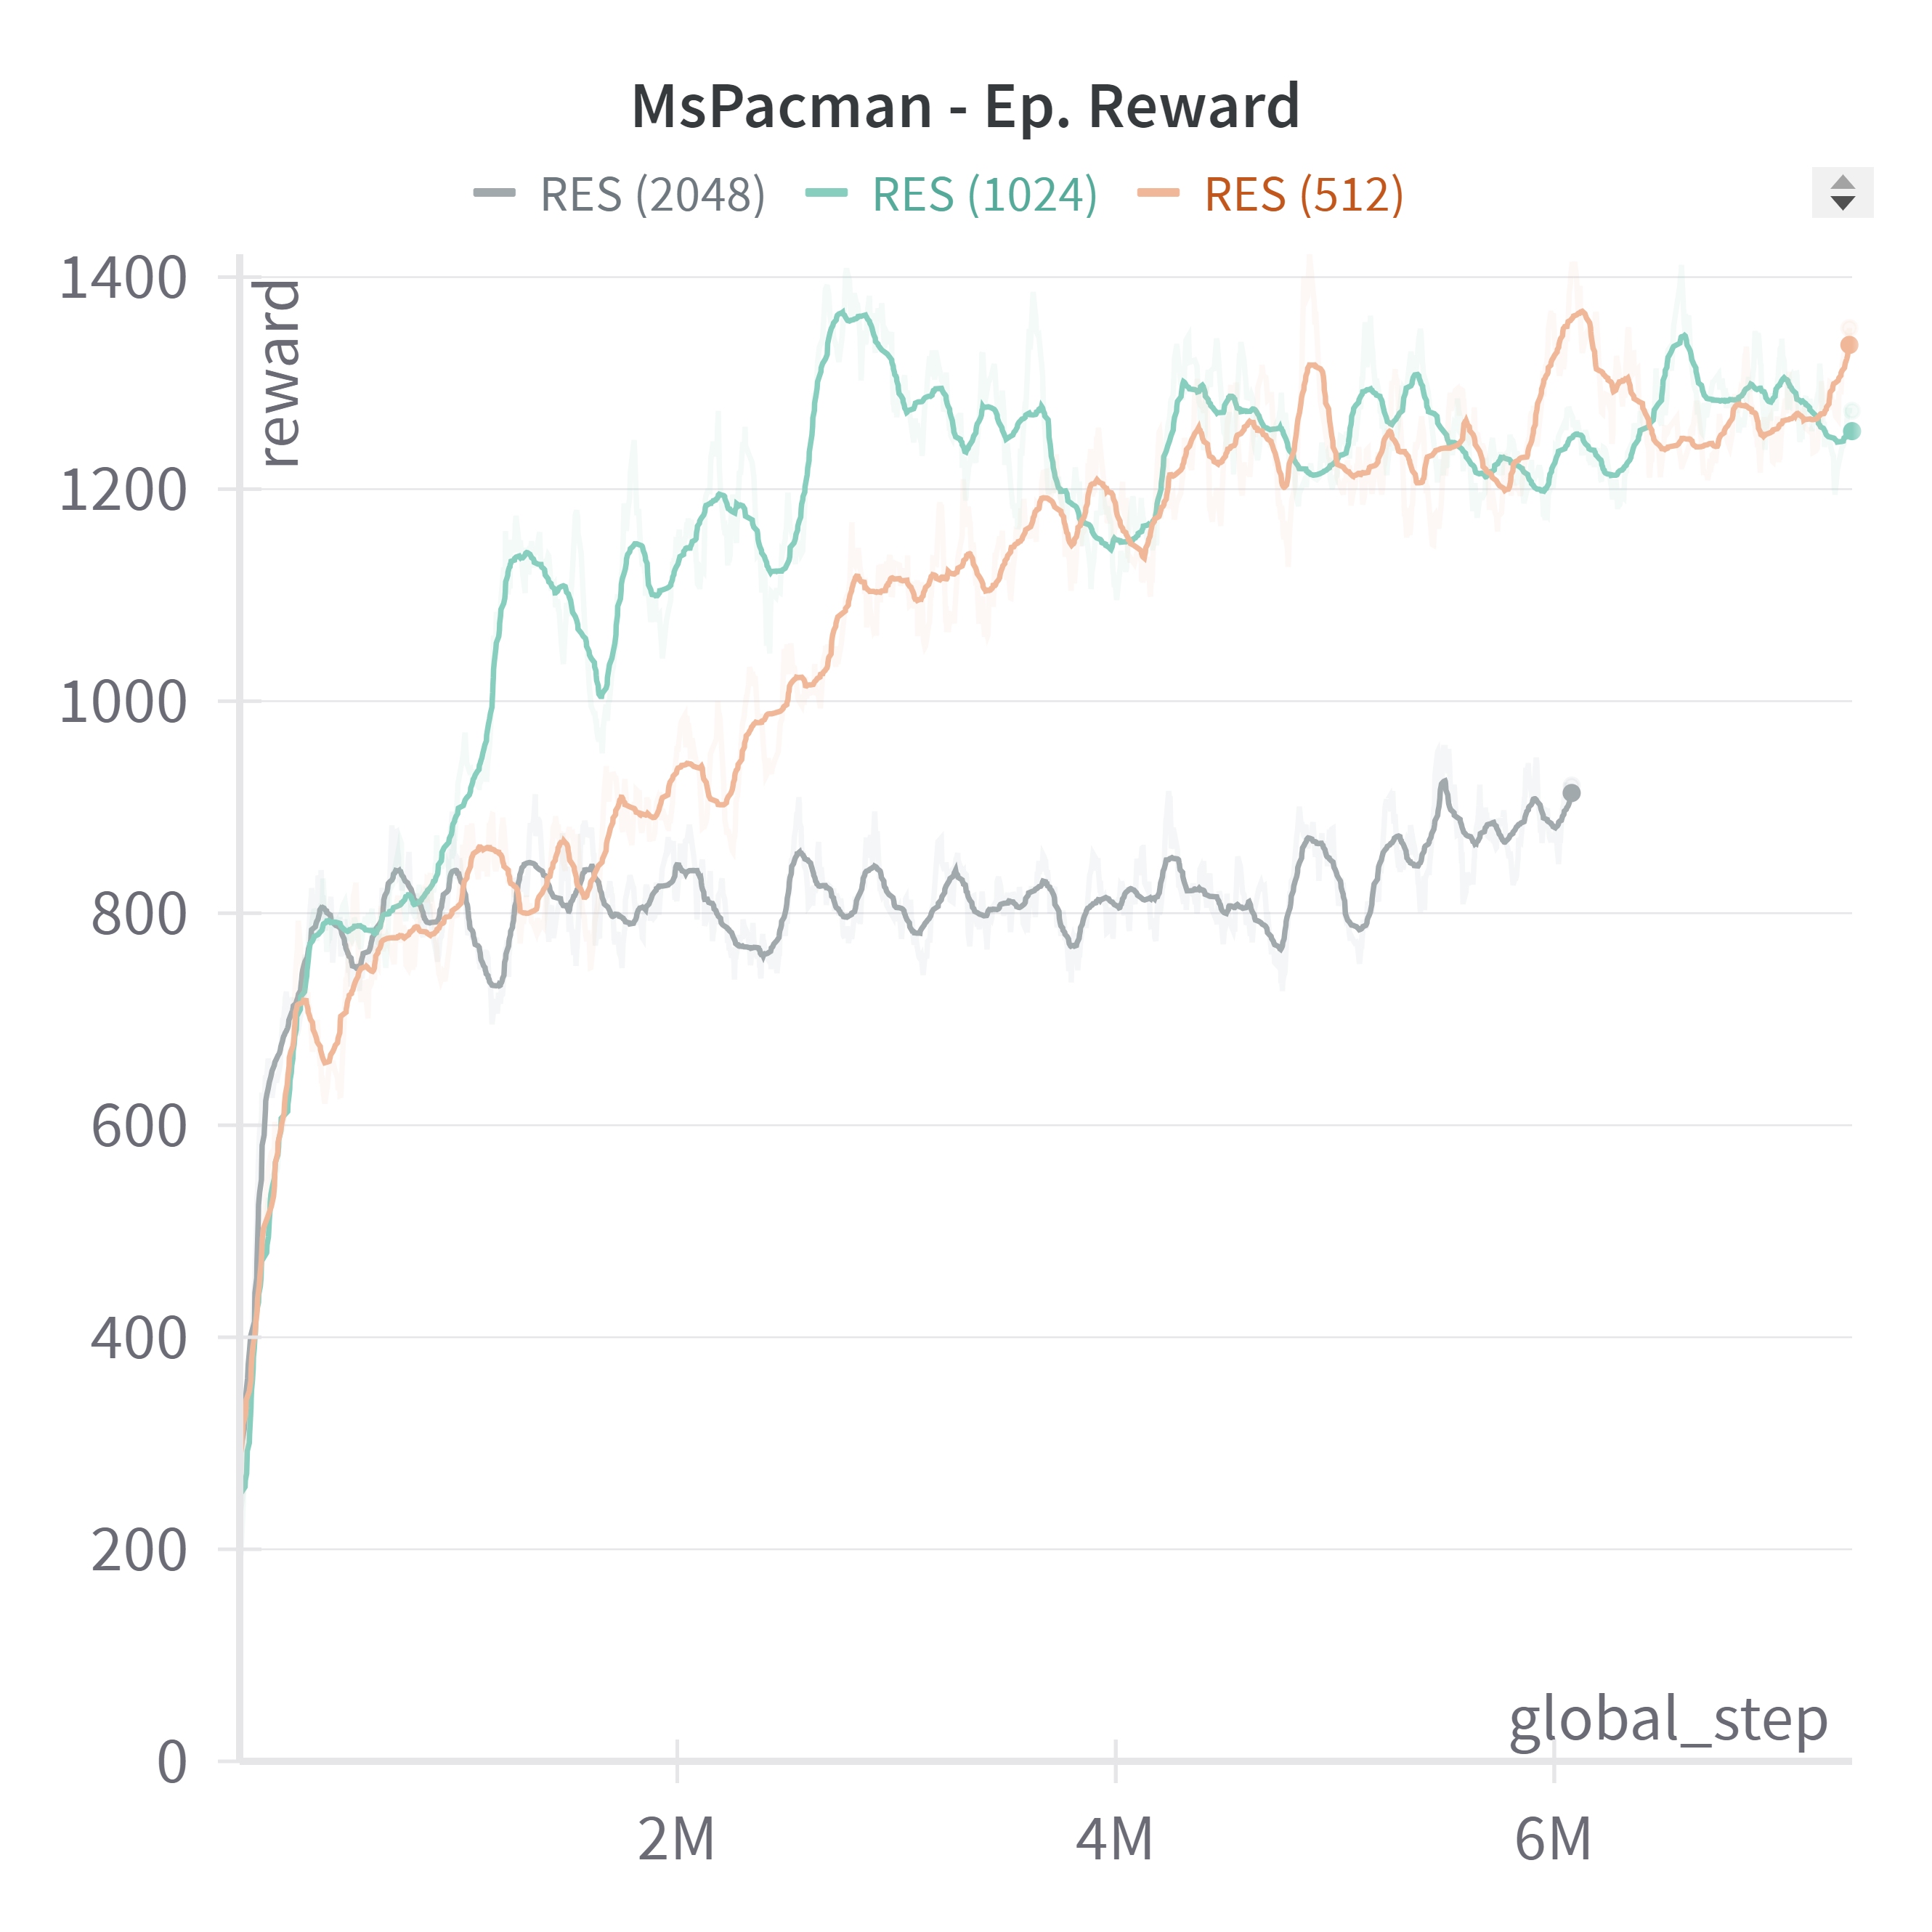
\includegraphics[width=\textwidth]{images/mspacman_res.png}
        \caption{\texttt{Reservoir}}
        \label{fig:mspacman_res}
    \end{subfigure}
    \caption{Initial analysis between different combination modules configurations on \texttt{Ms.Pacman}.}
    \label{fig:mspacman_concat_modules}
\end{figure}

% breakout
\begin{figure}[ht]
    \centering
    \begin{subfigure}[b]{0.45\textwidth}
        \centering
        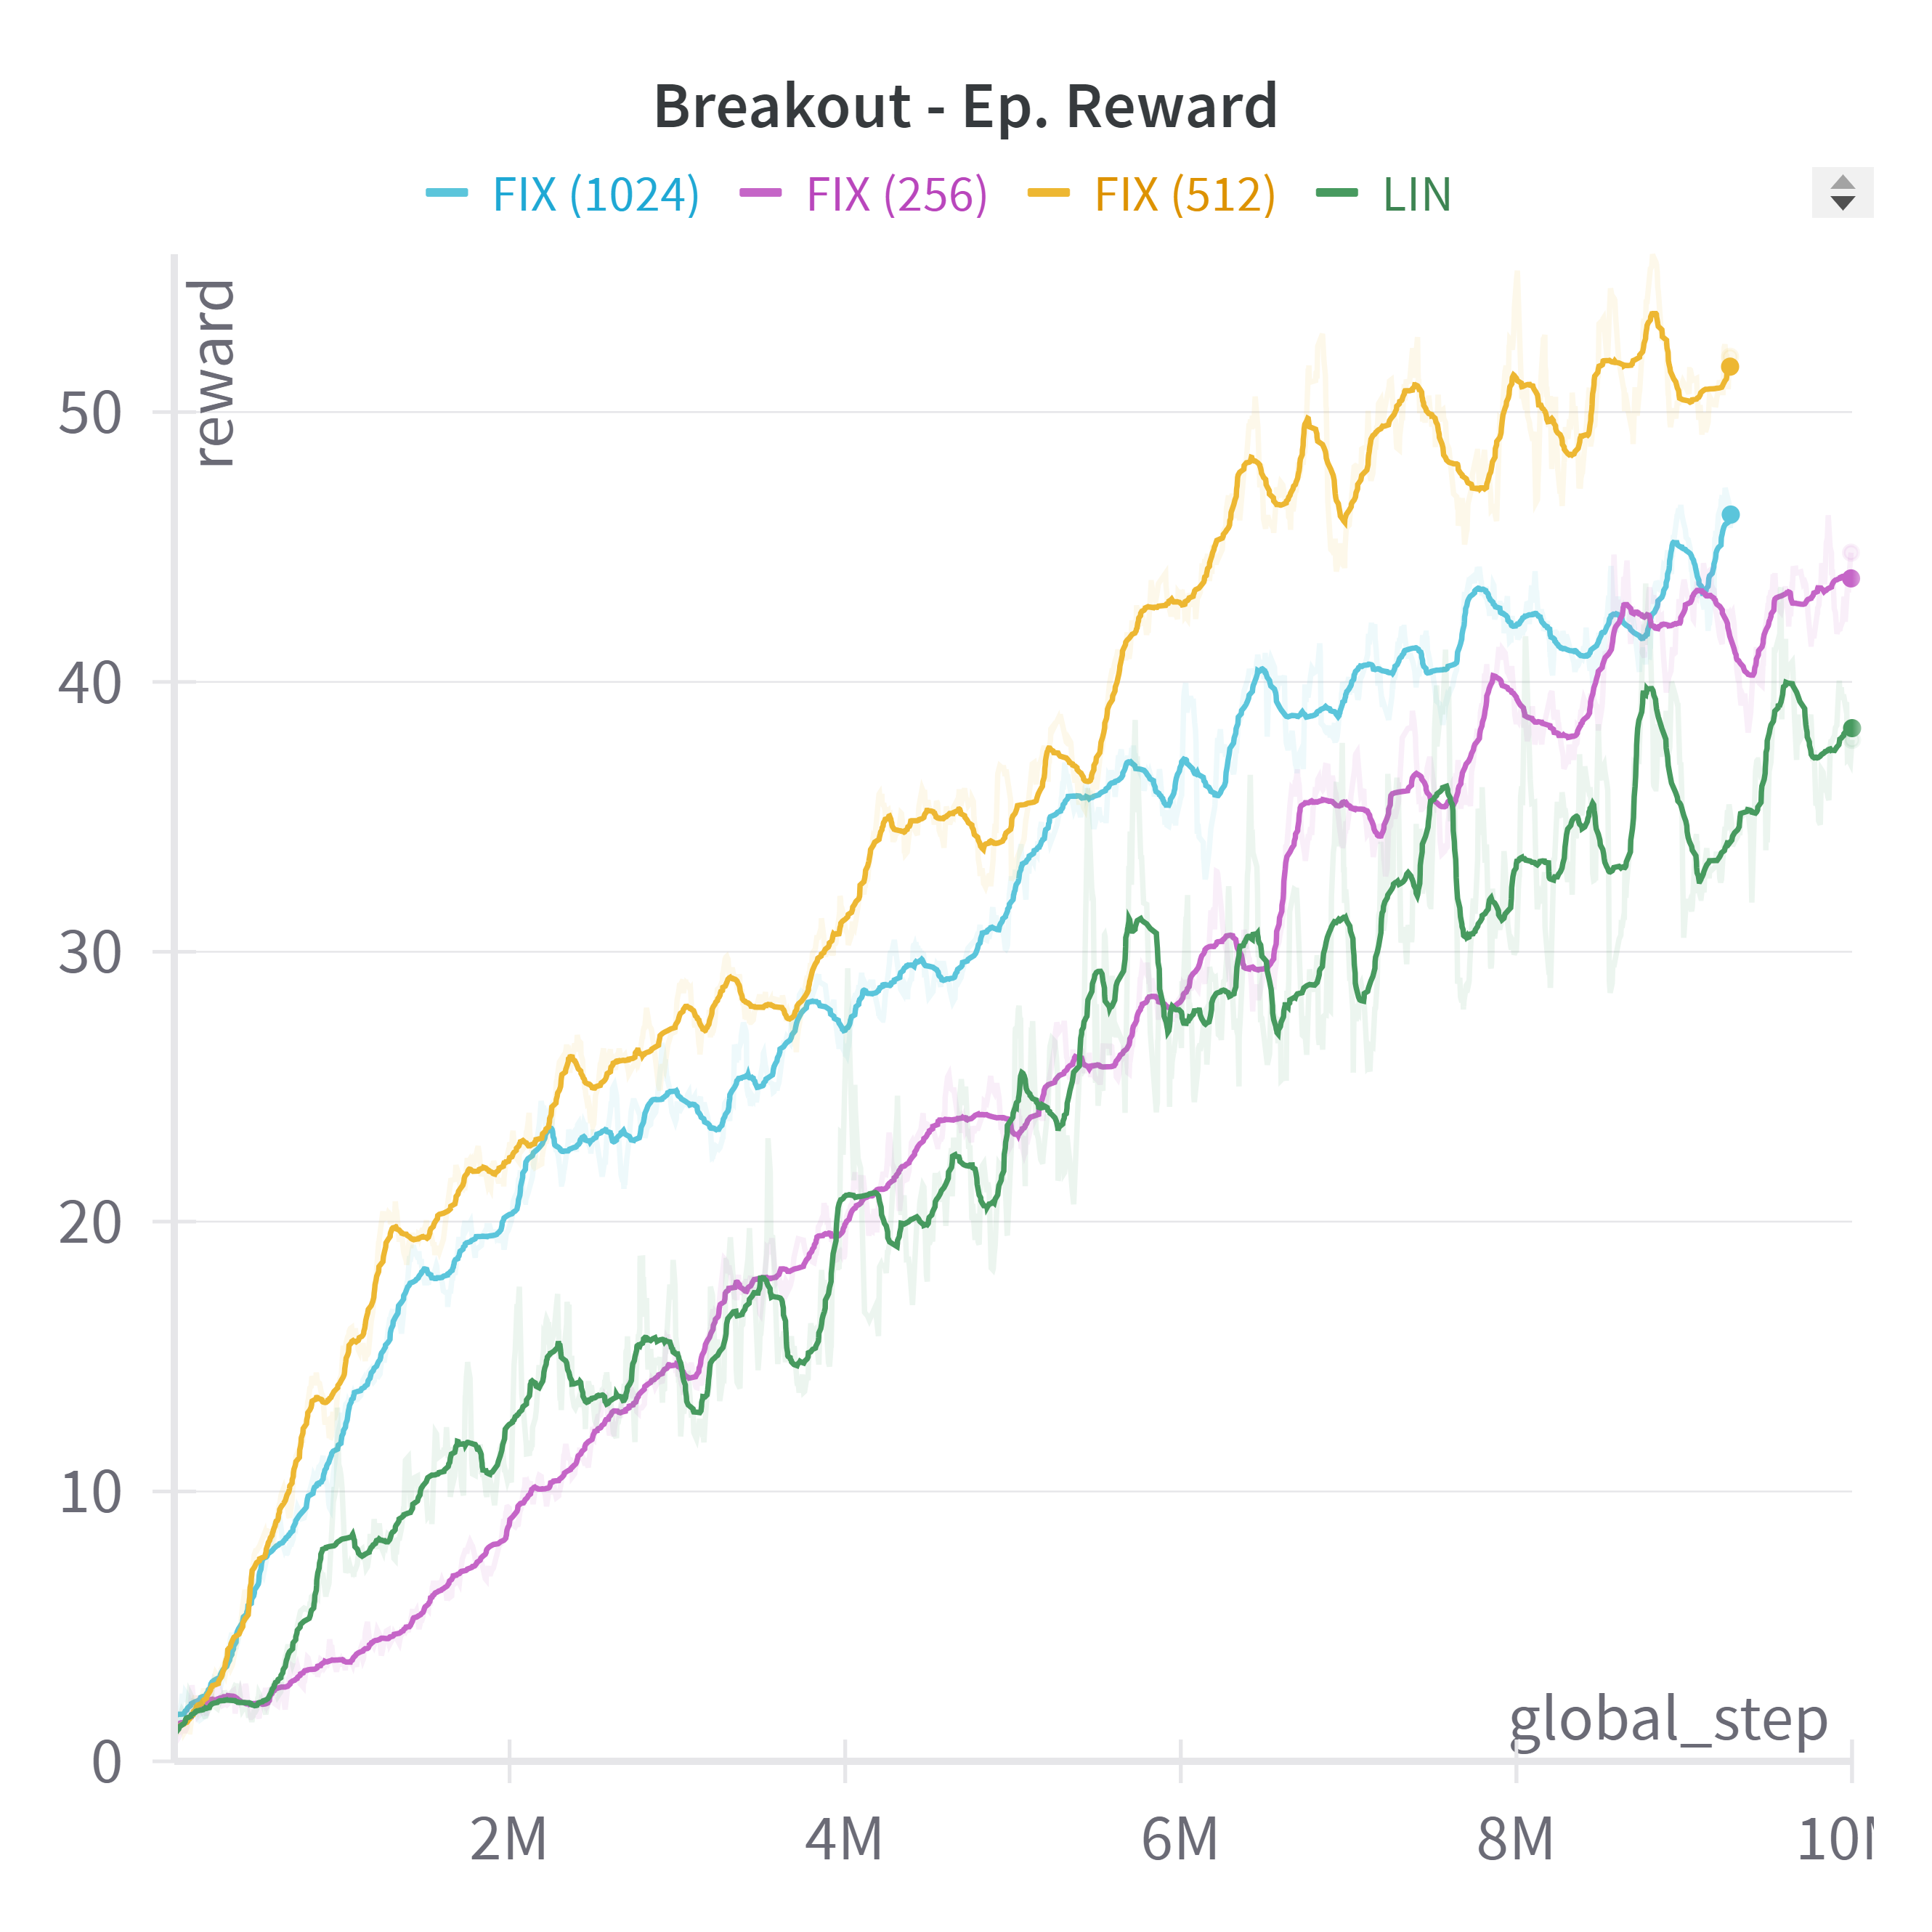
\includegraphics[width=\textwidth]{images/breakout_fix_lin.png}
        \caption{\texttt{Linear} and \texttt{Fixed Linear}}
        \label{fig:breakout_lin_fix}
    \end{subfigure}
    \hfill
    \begin{subfigure}[b]{0.45\textwidth}
        \centering
        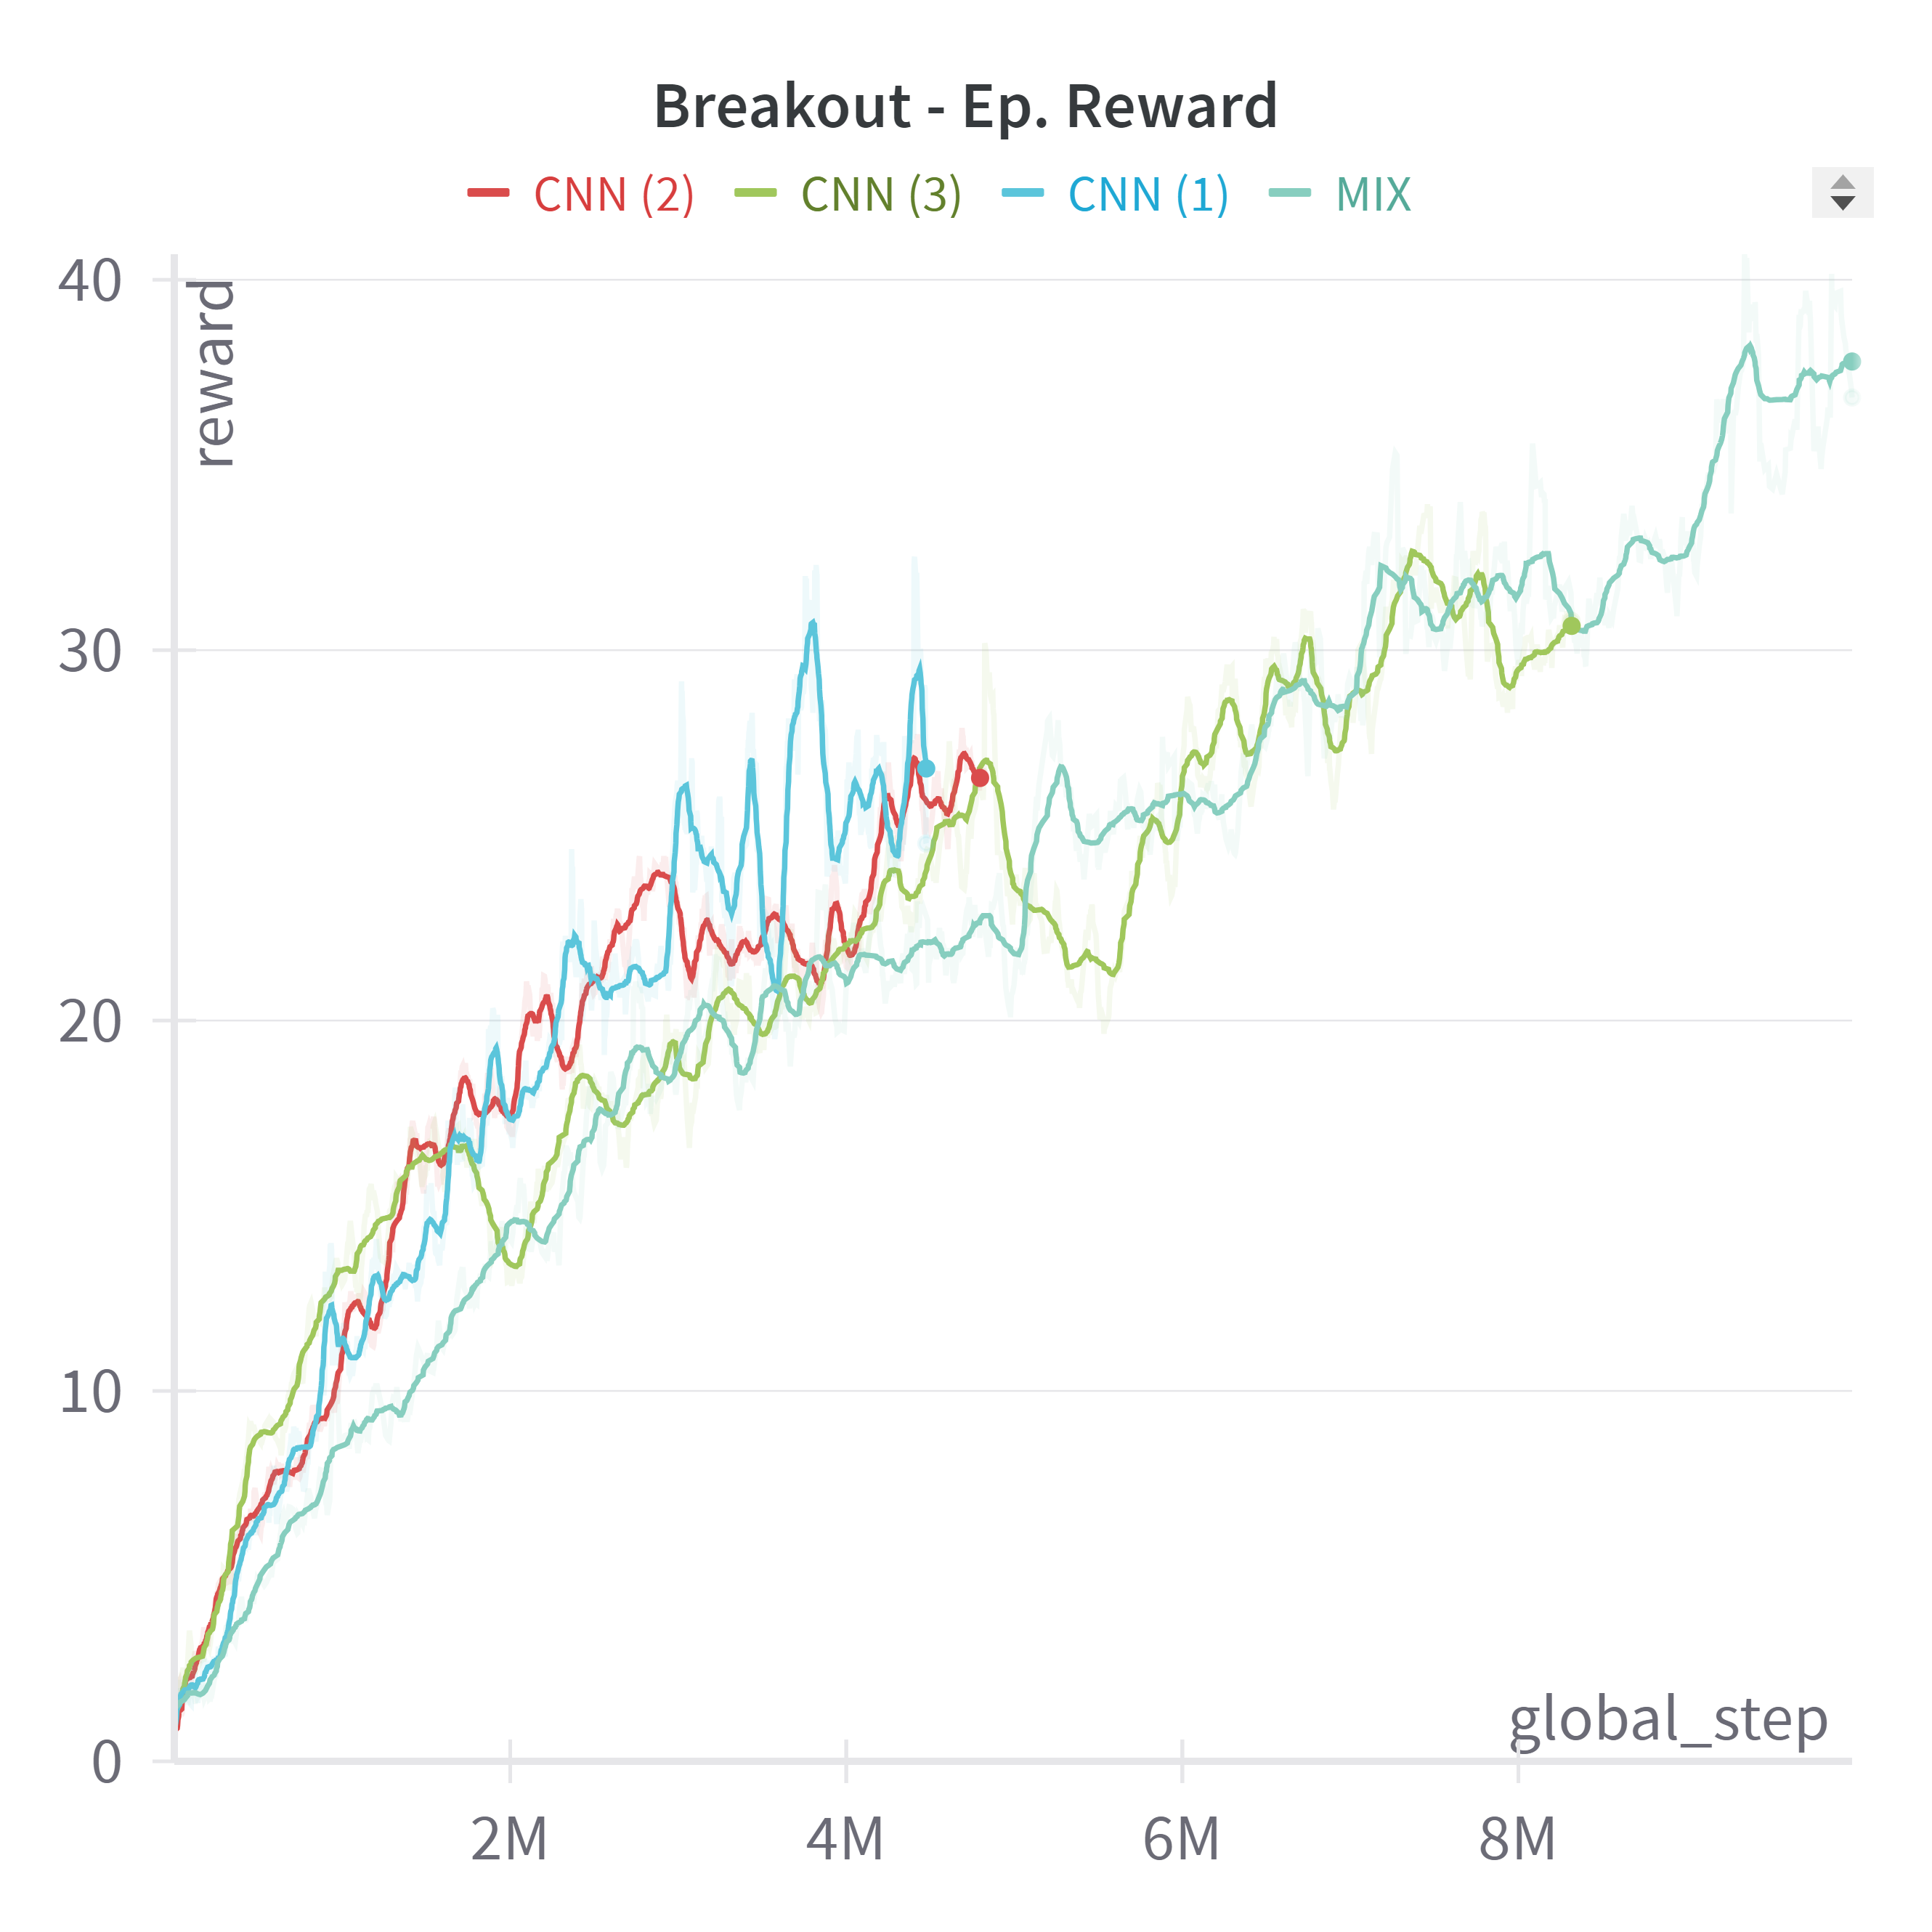
\includegraphics[width=\textwidth]{images/breakout_cnn_mix.png}
        \caption{\texttt{Convolutional} and \texttt{Mixed}}
        \label{fig:breakout_cnn_mix}
    \end{subfigure}
    \hfill
    \begin{subfigure}[b]{0.45\textwidth}
        \centering
        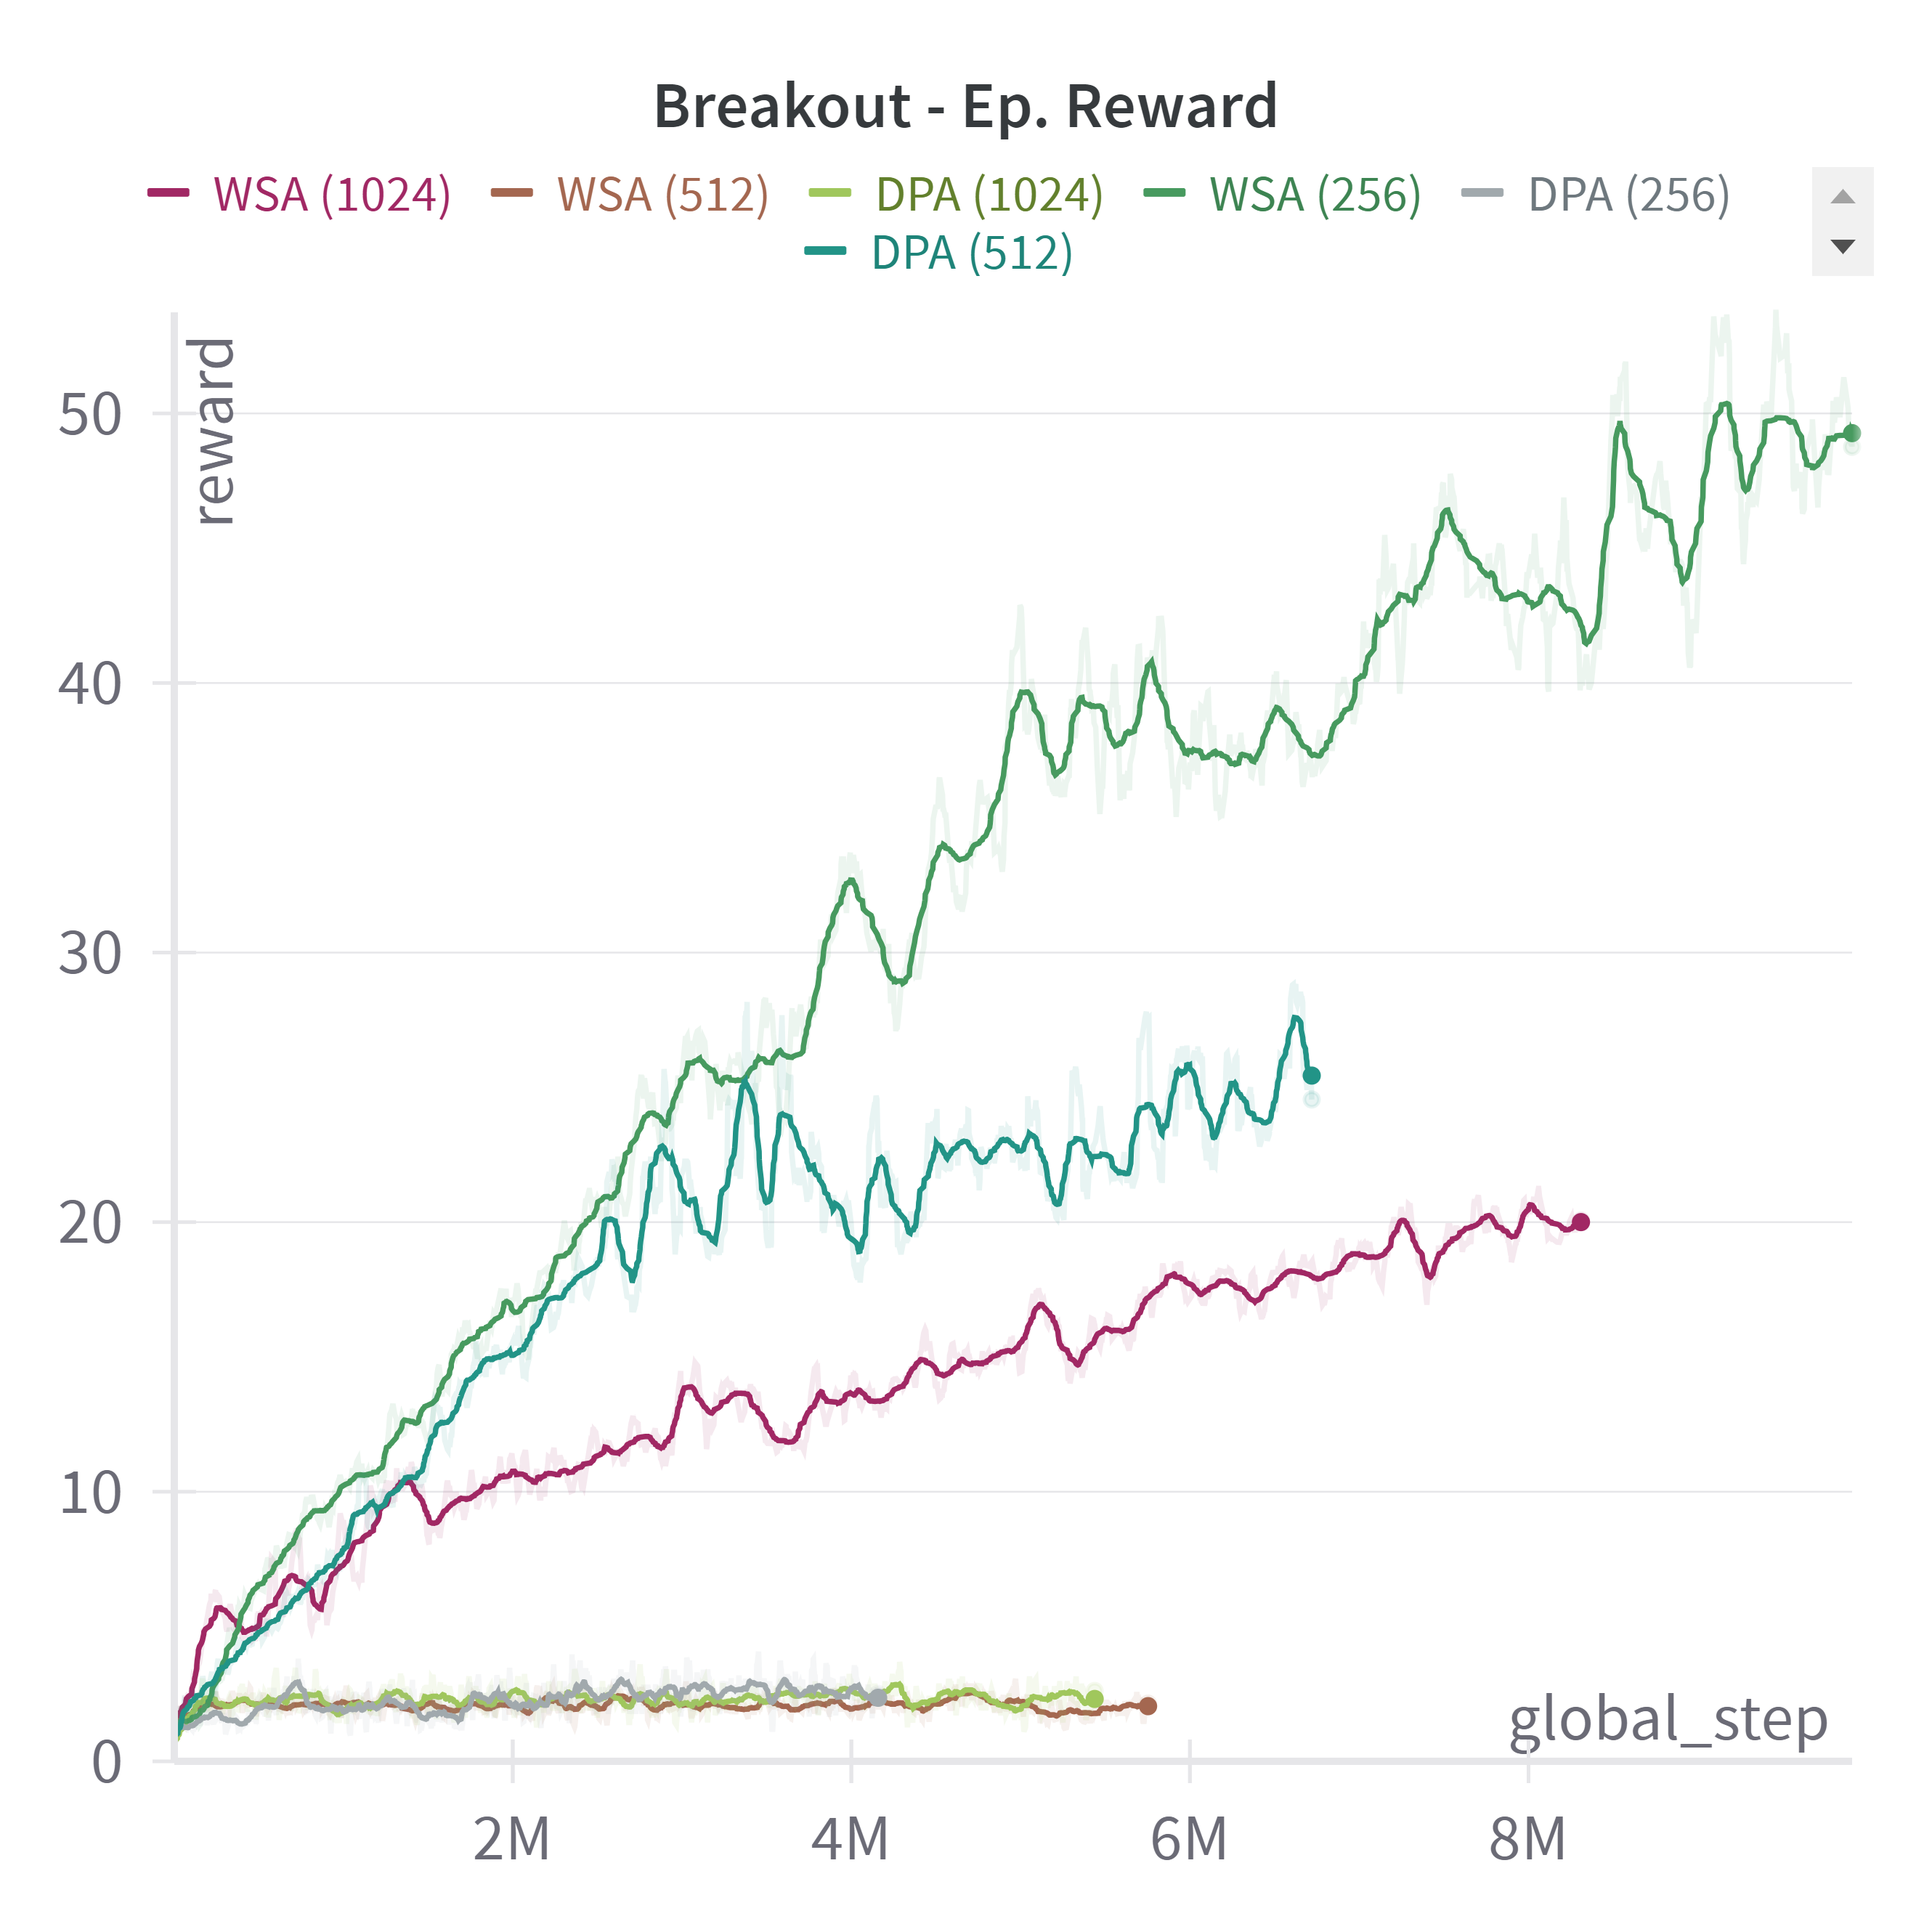
\includegraphics[width=\textwidth]{images/breakout_wsa_dpa.png}
        \caption{\texttt{Weight Sharing Attention} and \texttt{Dot Product Attention}}
        \label{fig:breakout_wsa_dpa}
    \end{subfigure}
    \hfill
    \begin{subfigure}[b]{0.45\textwidth}
        \centering
        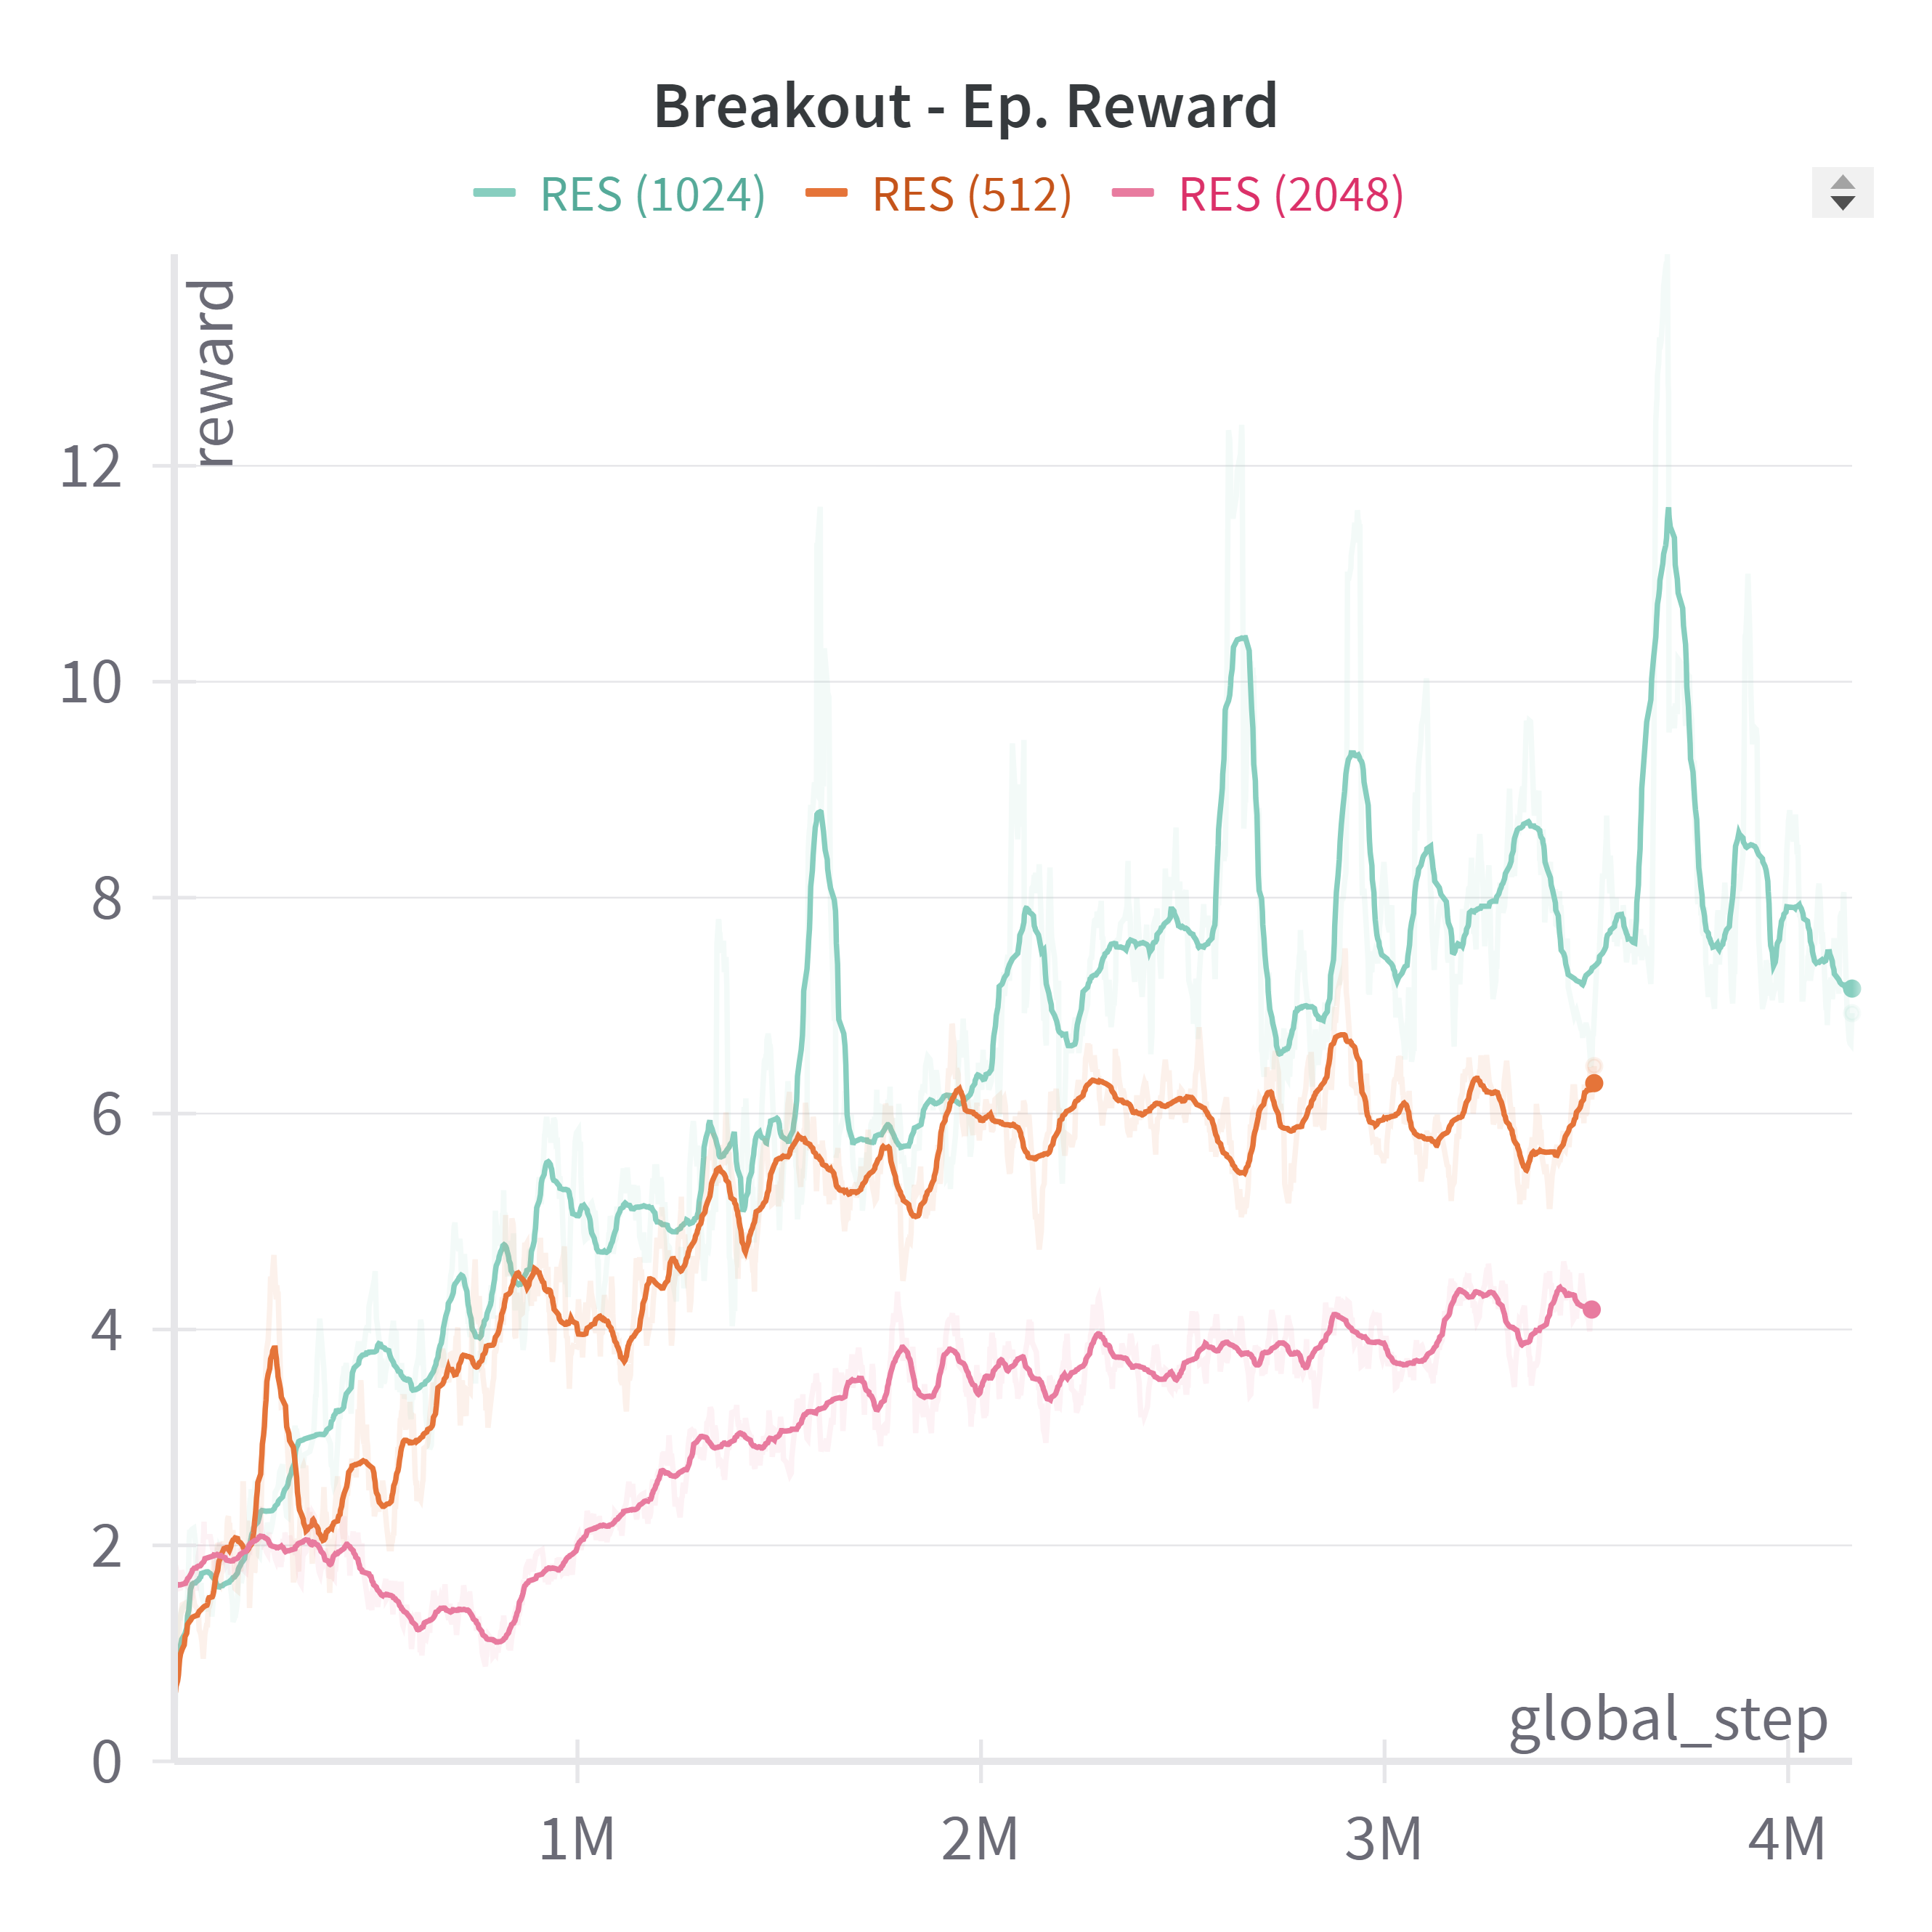
\includegraphics[width=\textwidth]{images/breakout_res.png}
        \caption{\texttt{Reservoir}}
        \label{fig:breakout_res}
    \end{subfigure}
    \caption{Initial analysis between different combination modules configurations on \texttt{Breakout}.}
    \label{fig:breakout_concat_modules}
\end{figure}